\documentclass[italian]{report}
\usepackage[italian]{babel}
\usepackage[utf8]{inputenc}
\usepackage{hyperref}
\usepackage{listings}

\title{
    Colture in cloud \\
    \large Applicazioni e Servizi Web
}

\author{
    Alex Baiardi - 0001041304 \{alex.baiardi@studio.unibo.it\}
    \and
    Giulio Zaccaroni - 0001025844 \{giulio.zaccaroni@studio.unibo.it\}
}
\date{12 Settembre 2022}

\usepackage{natbib}
\usepackage{graphicx}

\begin{document}
\maketitle
\tableofcontents

\chapter{Introduzione}
Il progetto nasce dall'esigenza di informatizzare alcuni processi di gestione della vendita diretta di una azienda agricola. In particolare, si vuole realizzare una soluzione software web-based che agevoli la memorizzazione e l'analisi dei dati relativi alle vendite.

Allo stato attuale l'azienda memorizza i dati in una base dati relazionale senza interfaccia grafica, l'obiettivo del progetto è quello di costruire un applicativo fruibile anche da utenti non esperti e sfruttare il cambiamento per innovare i processi aggiungendo funzionalità nuove.

La funzione principale è quella di memorizzare nuovi ordini tenendo traccia dei prodotti venduti, le rispettive quantità, i prezzi praticati ed eventualmente il cliente che ha acquistato. Inoltre si prevede la possibilità di avere più punti vendita a cui associare gli ordini e su cui effettuare l'analisi dei dati attraverso grafici.

Si prevede l'accesso al sistema  con diversi livelli di privilegio. In particolare, si può accedere ad un punto vendita come commesso o gestore. L'utente commesso potrà gestire gli ordini e i clienti, mentre l'utente gestore oltre ai privilegi del commesso potrà effettuare anche l'analisi dei dati. L'utente con i massimi privilegi è l'amministratore del sistema che gestisce punti vendita, prodotti e utenti. Inoltre ha la possibilità di effettuare l'analisi dei dati in forma aggregata su tutti i punti vendita.

\chapter{Requisiti}
Questo capitolo ha come scopo quello di descrivere dettagliatamente tutti i requisiti del software implementato. In particolare, si riporta l'elenco dei requisiti richiesti dall'azienda prodotto nelle prime fasi del progetto su cui si è basata la progettazione e lo sviluppo del software.
\section{Requisiti funzionali}
\begin{enumerate}
  \item L’utente accede al sistema inserendo nome utente e password.
  \item Il commesso di un punto vendita deve poter aggiungere, modificare e cancellare un cliente. Di un cliente si conosce denominazione e i seguenti dati opzionali: indirizzo, numero di telefono e partita iva.
  \item Il commesso di un punto vendita deve poter aggiungere un ordine inserendo data, il prezzo totale, le note (opzionali), un cliente (opzionale) ed uno o più articoli dove ogni articolo ha un prezzo, una quantità e eventualmente la qualità.
  \item Il commesso può modificare e cancellare gli ordini da lui inseriti.
  \item Il gestore di un punto vendita deve poter modificare e cancellare tutti gli ordini a cui ha accesso.
  \item I prezzi inseriti non includono le imposte.
  \item Il gestore di un punto vendita deve poter effettuare le azioni del commesso.
  \item Il gestore di un punto vendita deve poter visionare un grafico che mostri il fatturato in base a prodotto o varietà.
  \item Il gestore di un punto vendita deve poter visionare un grafico che mostri la quantità venduta in base a prodotto o varietà.
  \item Il gestore di un punto vendita deve poter visionare un grafico che mostri l'andamento delle vendite con possibilità di filtrare per: periodo di tempo, prodotto, varietà e cliente.
  \item Il gestore del sistema deve poter aggiungere e eliminare utenti.
  \item Il gestore del sistema deve poter agire anche come gestore dei singoli punto vendita.
  \item Il gestore del sistema deve poter aggiungere e modificare un punto vendita inserendo il nome e chi vi ha accesso.
  \item Il gestore del sistema deve poter aggiungere e modificare i prodotti inserendo nome, varietà disponibili (0 o più), unità di misura ed un prezzo consigliato (opzionale).
  \item Il gestore del sistema deve poter eliminare un prodotto nel caso in cui questo non abbia varietà assegnate.
  \item Il gestore del sistema per ogni prodotto deve poter aggiungere le varietà inserendo nome e prezzo consigliato (opzionale) ed eliminarle.
  \item Il gestore del sistema deve poter vedere grafici con dati aggregati per tutti i punti vendita.
  \item Ogni utente può visualizzare i propri dati e cambiare la password in completa autonomia.
  \item Il sistema deve tenere traccia di chi inserisce, modifica o elimina: ordini, clienti, prodotti e utenti.
\end{enumerate}
\section{Requisiti non funzionali}
\begin{enumerate}
    \item L’implementazione del sistema all’interno di un punto vendita deve risultare semplice e non invasiva.
    \item L'applicativo sviluppato deve essere accessibile anche a non vedenti e non udenti.
    \item L'aggiornamento dei dati deve avvenire automaticamente con un ritardo massimo nell'ordine dei secondi.
    \item L’interazione degli utilizzatori con il sistema deve avvenire in tempi ragionevoli.
    \item Il sistema deve essere progettato in modo da rendere il più semplice possibile la manutenzione.
\end{enumerate}
\section{Requisiti GDPR}
Per rispettare la vigente normativa GDPR è necessario:
\begin{itemize}
    \item Trattare i dati in modo lecito per finalità esplicite e determinate: nome utente e password sono utilizzati solo per l’autenticazione.
    \item Non dare la possibilità di collegare direttamente i dati all’interessato senza informazioni aggiuntive (pseudonimizzazione).
    \item I dati devono essere pertinenti e limitati (minimizzazione).
    \item Conservare i dati per il tempo necessario al conseguimento delle finalità per cui sono stati raccolti.
    \item Garantire la sicurezza e protezione dei dati.
    \item Non permettere il trasferimento dei dati extra-UE.
    \item Protezione dei dati memorizzati e scambiati nel sistema.
\end{itemize}
\chapter{Design}
Nella progettazione dell'applicazione ci si è concentrati sulle esigenze degli utenti cercando di ottenere un prodotto con una buona User Experience.
Il processo di design del sistema è stato di tipo partecipativo, in cui sono stati coinvolti alcuni utenti finali nell'evoluzione di tutto il progetto, in particolare sono state fatte varie riunioni con gli utenti finali del sistema. L'approccio utilizzato risulta essere di tipo \textbf{Co-creation} in cui gli utenti target sono stati coinvolti nelle fasi di definizione dei requisiti e design delle interfacce grafiche, ottenendo feedback continui.

\section{Design interfaccia utente}
Nella progettazione delle interfacce grafiche si è cercato di aderire agli standard e consuetudini in uso in questo campo (tra cui WCAG per quanto concerne l'accessibilità). Si è cercato di seguire una struttura delle pagine coerente e l'utilizzo di simboli noti per le principali funzioni. Inoltre 
ci si è allineati ai principi \textbf{KISS} e \textbf{"Less is More"} con l’obiettivo di realizzare una interfaccia semplice ed intuitiva nell’utilizzo da parte degli utenti. Un altro importante principio che è stato seguito è quello del \textbf{Responsive Design}, affinché non vi siano vincoli su quale dispositivo utilizzare.
\subsection{Mockup}
Per dare forma all'applicazione e definire al meglio tutti i requisiti, sono stati realizzati alcuni mockup delle schermate principali.
I mockup sono stati realizzati attraverso l'editor \textbf{Figma} che ci ha permesso di realizzare delle interfacce fedeli al risultato finale da mostrare ai committenti. Questo è molto importante affinché gli utenti finali possano avere una idea precisa del risultato e quindi fornire buoni feedback.

\begin{figure}[htp]
    \centering
    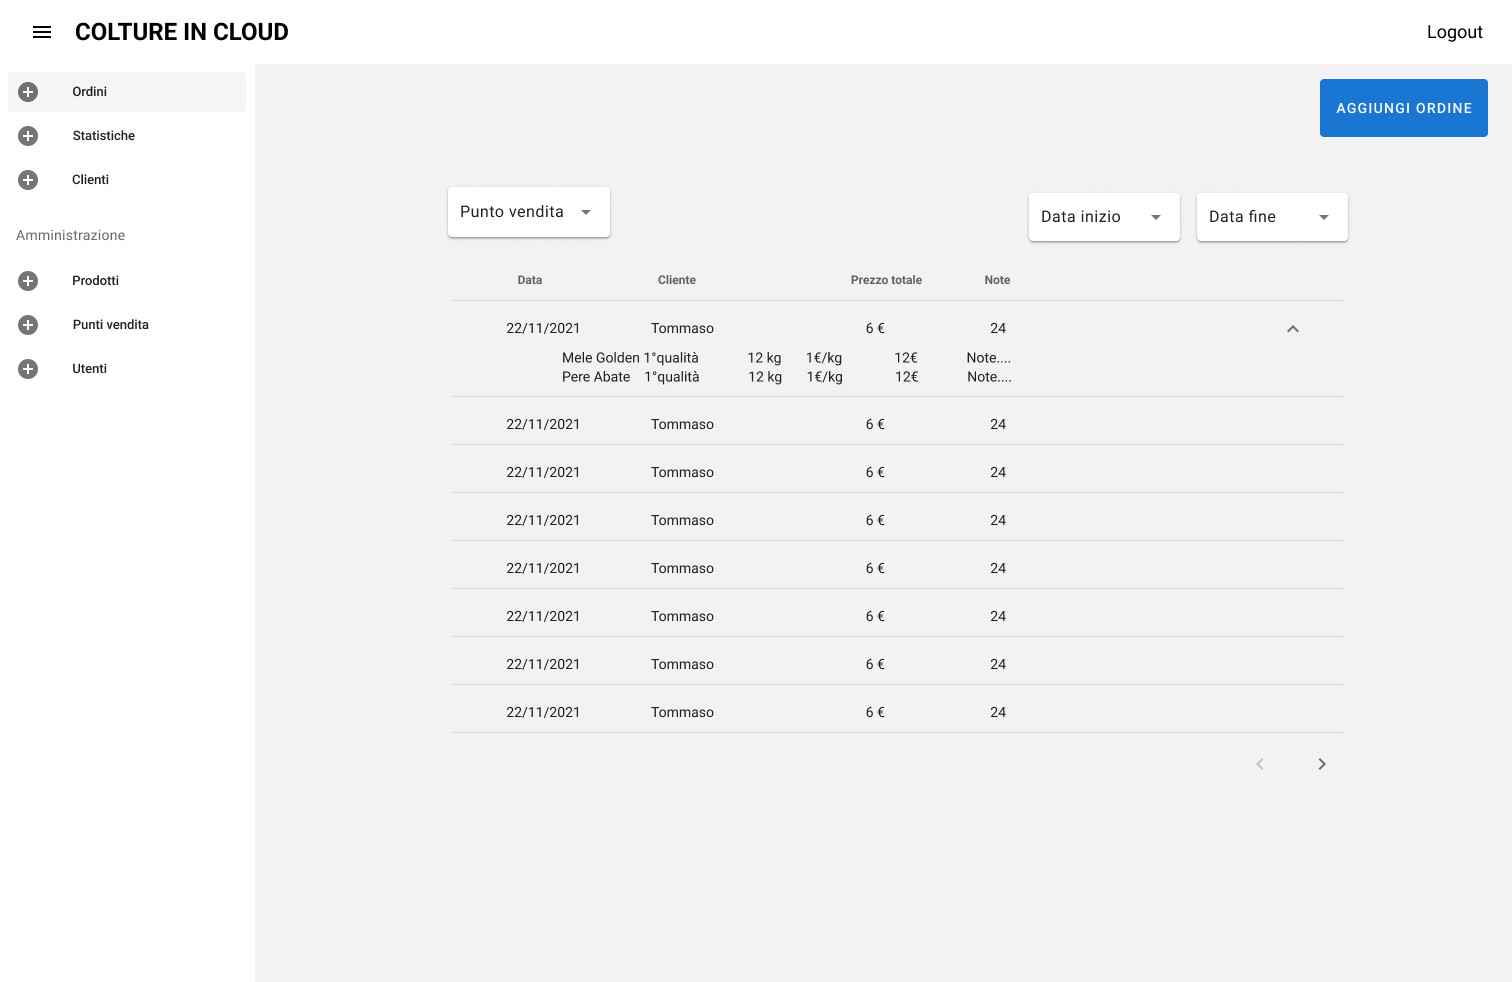
\includegraphics[width=\textwidth]{assets/mockup_orders.jpg}
    \caption{Mockup gestione ordini}
    \label{fig:getOrders}
\end{figure}
\begin{figure}[htp]
    \centering
    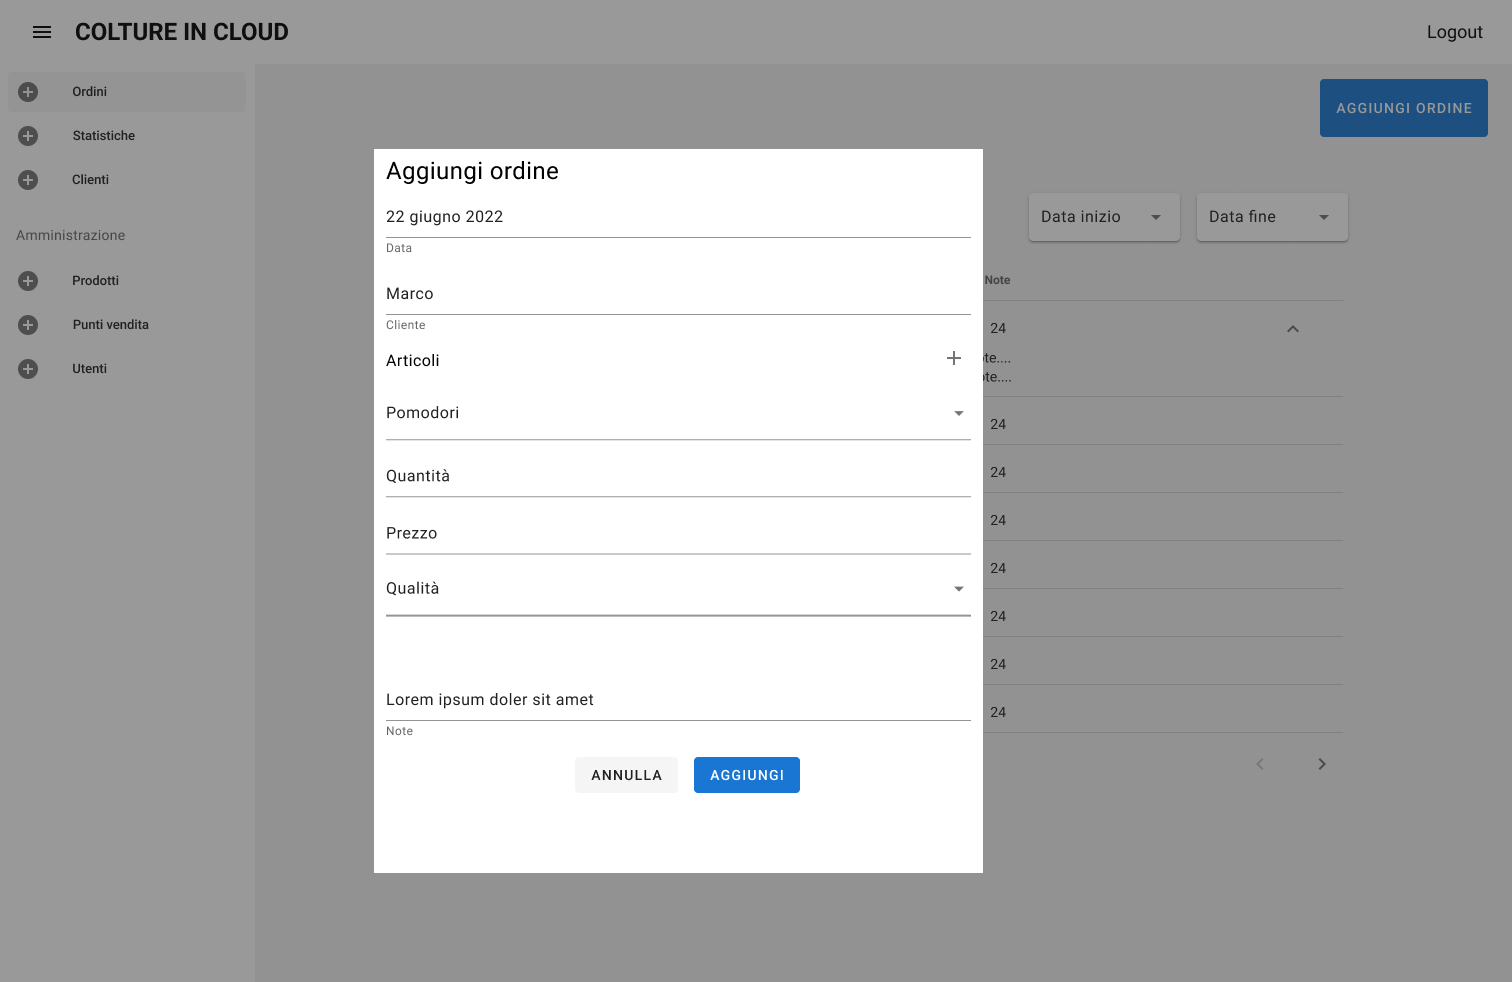
\includegraphics[width=\textwidth]{assets/mockup_add_order.jpg}
    \caption{Mockup creazione nuovo ordine}
    \label{fig:addOrder}
\end{figure}
\begin{figure}[htp]
    \centering
    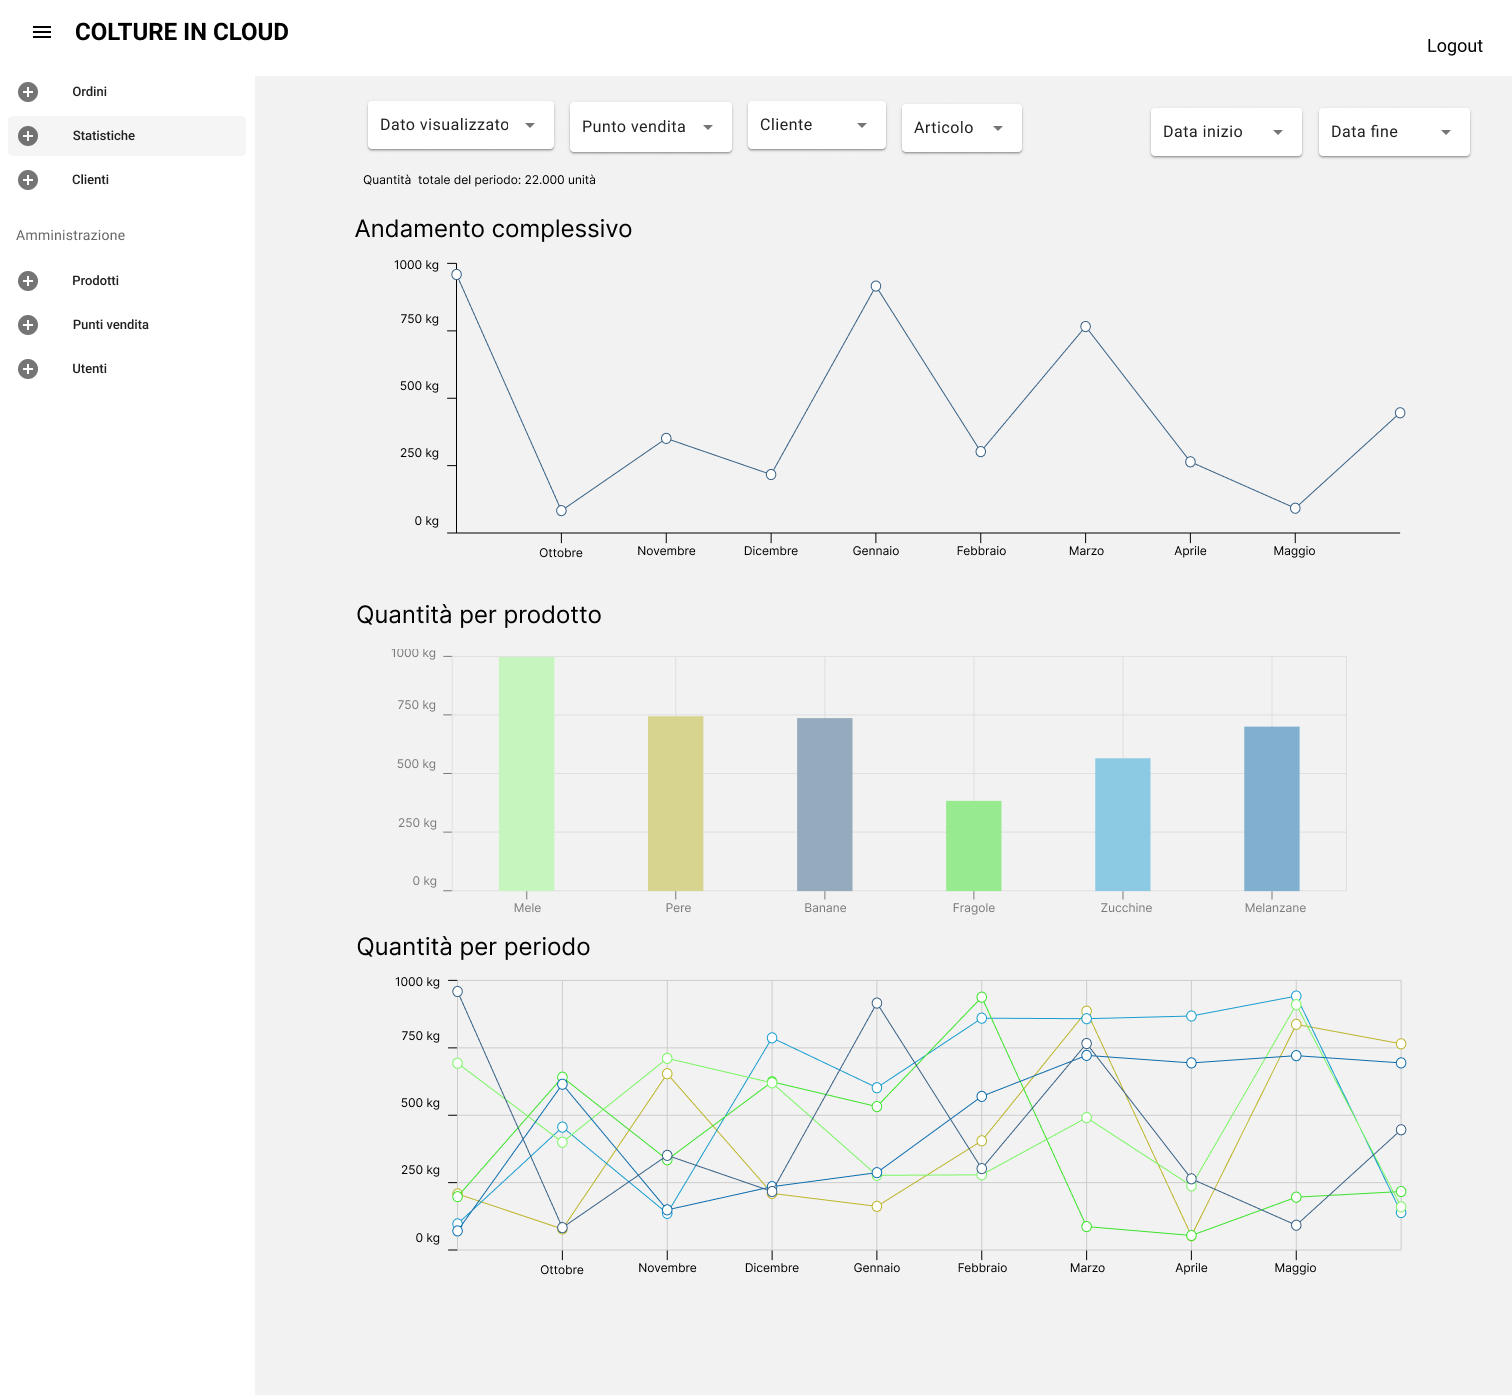
\includegraphics[width=\textwidth]{assets/mockup_stats.jpg}
    \caption{Mockup visualizzazione statistiche}
    \label{fig:analytics}
\end{figure}
\begin{figure}[htp]
    \centering
    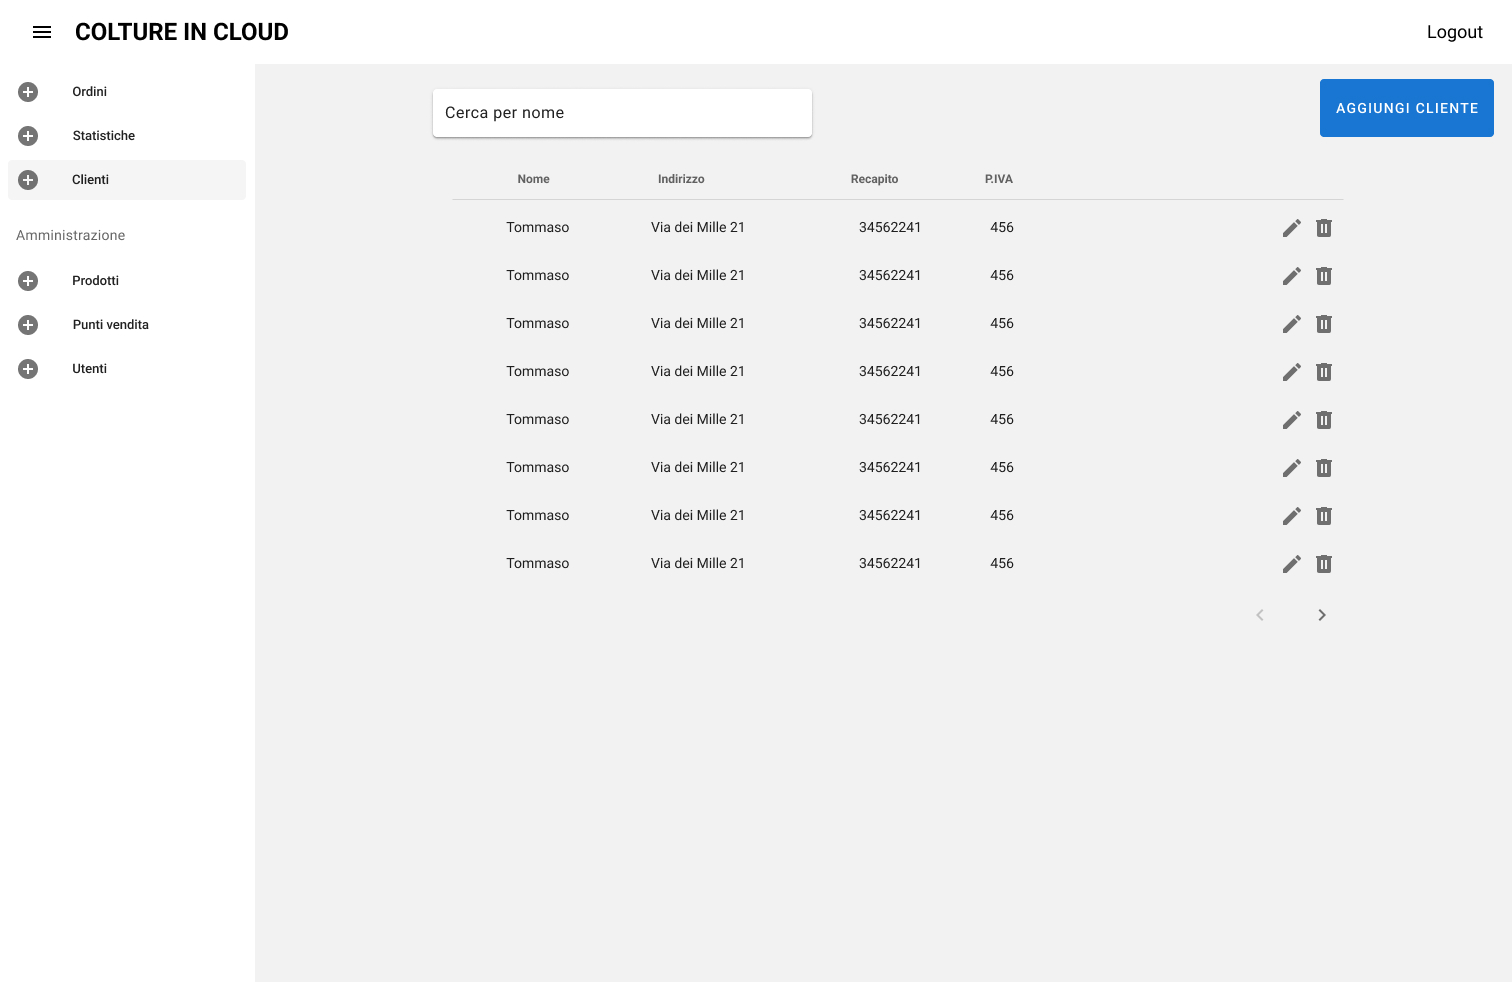
\includegraphics[width=\textwidth]{assets/mockup_customers.jpg}
    \caption{Mockup gestione clienti}
    \label{fig:getClients}
\end{figure}
\begin{figure}[htp]
    \centering
    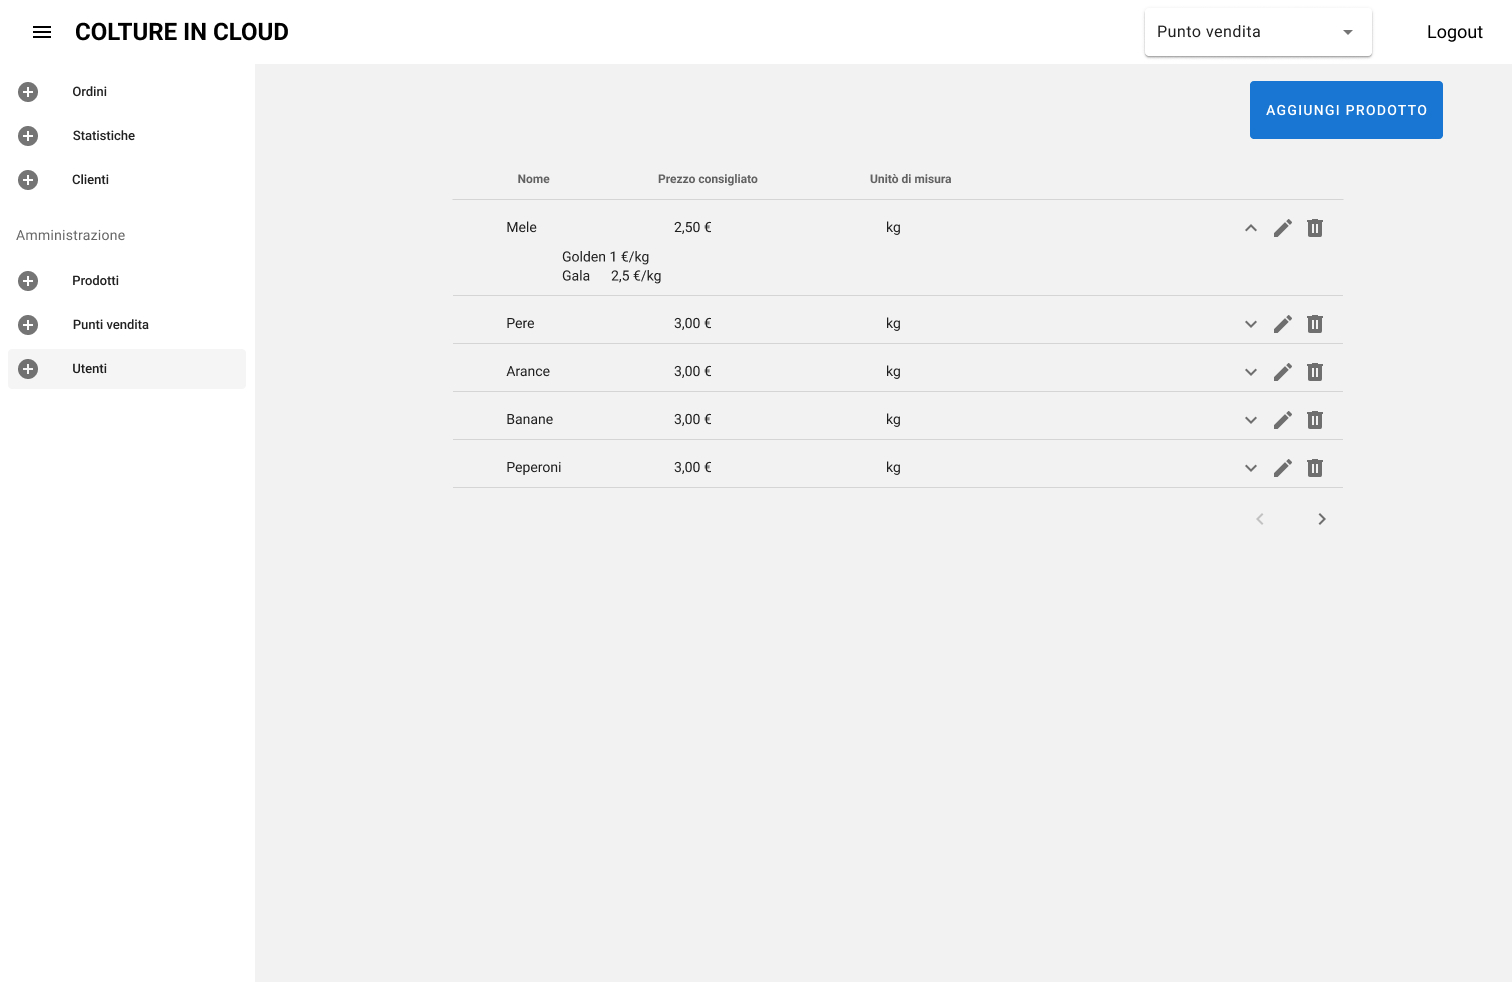
\includegraphics[width=\textwidth]{assets/mockup_products.jpg}
    \caption{Mockup gestione prodotti}
    \label{fig:getProducts}
\end{figure}

\section{Design dell'architettura del sistema}
L'applicativo si compone di 
\begin{itemize}
    \item backend: si occupa di gestire la business logic, il salvataggio ed il recupero dei dati;
    \item frontend: il quale si occupa di gestire la visualizzazione dei dati e l'interazione con l'utente.
\end{itemize}
Il disaccoppiamento tra i due porta a una divisione tra una componente statica (il frontend) e una componente dinamica (stateless). \\
L'interazione tra backend e frontend avviene tramite una API REST-ful predefinita in modo da consentire uno sviluppo indipendente delle componenti del sistema. Questa API ci permette di disaccoppiare il modo di rappresentazione dei dati all'interno della base di dati dal modo di trasmissione in rete. Ad esempio, in futuro potrebbero essere introdotte nuove versioni dell'API che supportano nuovi formati di dati senza necessariamente dover modificare la struttura della base di dati. 

Le API sono state descritte attraverso \textbf{OpenAPI} che fornisce un metodo standard e rigoroso per la descrizione di API REST.
È possibile reperire la documentazione dell'API a \href{https://app.swaggerhub.com/apis/ZACCARONIGIULIO/ColtureCloud/1.0.0}{questo indirizzo}.\\
Sia backend sia frontend condividono un modulo in comune che si occupa di:
\begin{itemize}
    \item validare i dati;
    \item mantenere il modello del sistema;
    \item mantenere la business logic in comune.
\end{itemize}
La persistenza è gestita tramite un database di tipo non-relazionale, portandoci ad alcuni accorgimenti in fase di design, tra cui:
\begin{itemize}
    \item ridondanza dei dati: non essendo relazionale è meglio salvare i dati collegati a un elemento con esso. Ad esempio: assieme a un ordine vengono anche salvati i dati del cliente e del punto vendita dove viene effettuato. Questo ci permette una più rapida visualizzazione dei dati e un minore utilizzo della base di dati.
    \item resistenza a inconsistenza: poiché in molti database non-relazionali non è consentito l'uso di transazioni atomiche su più documenti il backend deve essere in grado di gestire anche una momentanea inconsistenza dei dati.
\end{itemize}

La scelta di utilizzare un database non relazionale è stata particolarmente significativa, in quanto è un cambiamento radicale rispetto al sistema esistente. Questo ci ha portato a ripensare totalmente il sistema precedente e fornire un supporto per migliorare i processi aziendali come richiesto dall'azienda che ha commissionato il lavoro. In questo modo si segue il concetto di Business Process Reengineering, in cui il sistema informatico aiuta a migliorare il business aziendale.

\chapter{Tecnologie}

Il sistema è stato realizzato utilizzando il \textbf{solution stack MEVN} tra i moderni stack di tecnologie Javascript-based per la realizzazione di Single Page Applications. La scelta di affidarsi a questo tipo di stack deriva dal fatto che permette di concentrarsi maggiormente su come implementare il sistema indipendentemente dalla piattaforma e definisce in modo completo come strutturarlo. Inoltre viene definita una netta separazione con adeguato supporto alla programmazione lato client e lato server, con la possibilità di riutilizzo del codice.

\subsection{Typescript}
Si è deciso di usare per l'intero applicativo il linguaggio di programmazione di Typescript, questo permette:
\begin{itemize}
    \item l'interoperabilità con Javascript attraverso la traduzione del codice;
    \item l'"auto-documentazione" del codice, l'utilizzo dei tipi rende molto più semplice capire il funzionamento di ogni metodo o variabile;
    \item una migliore integrazione con gli editor di testo;
    \item l'utilizzo di funzioni Javascript non ancora disponibili sui browser (e.g. è possibile usare async/await anche se la versione di javascript usata dal browser non lo supporta).
\end{itemize}

\section{Backend}
Il sistema lato server è formato da un servizio backend basato su Node.js con Express.js come framework di gestione delle richieste e un layer di persistenza implementato da un database non relazionale con motore MongoDB. Questo tipo di database permette una gestione molto meno rigida dei dati e risulta più facile da mantenere e modificare, inoltre, presentando i dati nel formato JSON, rende più semplice la programmazione che non necessita di particolari aggiustamenti dei dati.

\subsection{Autenticazione}
Per gestire l'autenticazione abbiamo deciso di utilizzare le sessioni:
\begin{itemize}
    \item ne viene creata una nuova ogni volta che un utente accede al servizio;
    \item vengono salvate nella base di dati, quindi, nel caso in cui ci siano più server a gestire il backend, funziona comunque;
    \item a differenza di Json Web Token, ci permette di revocare immediatamente l'accesso di un determinato utente alla piattaforma evitando la presenza di dati vecchi (stale) nel token;
    \item comporta un maggiore utilizzo della base di dati sia per il salvataggio della sessione, sia per il recupero delle informazioni relative all'utente.
\end{itemize}

\subsection{Socket.io}
Per l'aggiornamento in tempo reale dei dati visualizzati attraverso il frontend abbiamo deciso di utilizzare Socket.io. Questa è una libreria JavaScript per le real-time web application che abilita la comunicazione bidirezionale in tempo reale tra client e server. È composta da due componenti: una client-side e una server-side per Node.js. L’idea di base è, quando si verifica un evento, notificare direttamente i client connessi interessati tramite il server i quali reagiscono eseguendo i listener registrati.

\subsection{MongoDb Atlas}
Per garantire la sicurezza e protezione dei dati come richiesto dal GDPR e al contempo minimizzare la manutenzione del servizio abbiamo scelto di usare MongoDb Atlas. Quest'ultimo:
\begin{itemize}
    \item è totalmente gestito direttamente da MongoDb;
    \item offre la possibilità di mantenere i server in Italia;
    \item offre l'encryption-at-rest quindi i dati sono criptati sul server;
    \item permette di connettersi mediante TLS;
    \item diminuisce in maniera drastica i tempi di deployment e mantenimento.
\end{itemize}
Ovviamente nel caso un cliente diverso in futuro non necessiti di rispettare questi requisiti è possibile usare anche una istanza MongoDb tramite Docker o altri servizi/fornitori.

\section{Frontend}
Il sistema è reso disponibile agli utenti tramite una interfaccia sviluppata con l'utilizzo di VueJS. Si è deciso di usare questo framework perché: supportato da una grande comunità di sviluppatori, più leggero di Angular e di più semplice apprendimento. Inoltre permette la creazione tramite Electron di app desktop a partire dalla stessa codebase nel caso in cui in un futuro ve ne fosse necessità.

\subsection{Vuetify}
Per l'implementazione della UI è stato scelto di usare una libreria che contenga già gran parte dei componenti necessari con supporto all'accessibilità. Questo ci ha permesso di essere molto più rapidi nello sviluppo ed evitare di "reinventare la ruota".
\subsection{Webpack}
Il frontend verrà utilizzato principalmente tramite web e questo impone vincoli sia a livello di compatibilità sia a livello di dimensioni del codice. Per rispettarli ed avere una applicazione il più possibile performante abbiamo deciso di usare Webpack, questo, attraverso il tree-shaking elimina il codice non utilizzato e permette di avere un'applicativo finale molto più leggero oltre a produrre codice retro-compatibile.
\subsection{Internazionalizzazione}
Quando si parla di accessibilità un aspetto spesso sottovalutato è quello dell'internazionalizzazione, infatti se il software è in una lingua diversa da quella dell'utente si crea una barriera e una difficoltà nell'utilizzo. Inoltre, internazionalizzare un software in un secondo momento è spesso molto oneroso in termini di tempo. Per questo abbiamo deciso di usare una libreria denominata I18N e abbiamo inserito tutti i testi in un file json dedicato allo scopo.

\chapter{Codice}
\section{Modularità}
Un aspetto fondamentale nello sviluppo di questa applicazione è stato quello di evitare duplicazioni:
\begin{itemize}
    \item nel codice scritto da noi;
    \item nei moduli importati da npm;
    \item nelle configurazioni dei vari servizi.
\end{itemize}
Per gestire al meglio questo aspetto abbiamo diviso in due macro-categorie i componenti del progetto: le "apps" ovvero i servizi avviabili e i "packages": i moduli condivisi tra le "apps".
Successivamente abbiamo configurato NPM in modo che capisse che era un unico progetto per evitare duplicazioni tramite l'utilizzo degli NPM Workspaces, questo va a creare un unica cartella \lstinline{node_modules} nella radice contenente tutti i moduli riducendo in maniera importante le duplicazioni. 
Infine, abbiamo configurato Typescript in modo che potesse leggere i file anche dai moduli in "packages" attraverso le Project References.
\section{Stile del codice}
Per uniformare lo stile del codice all'interno del progetto abbiamo usato ESLint con Prettier, questo ci ha consentito di avere un codice molto più leggibile, pulito e di evitare bad-practices attraverso l'uso dei consigli di ESLint.
Inoltre, dato che Javascript non supporta direttamente gli import assoluti portando a import poco leggibili come \lstinline{"../../../../../model/Casa.ts"} abbiamo abilitato il supporto ad essi attraverso l'uso di appositi moduli  che permettono la scrittura di \lstinline{@/model/Casa.ts} andando poi a tradurli nel formato accettato da Javascript. 

\chapter{Test}
Le funzionalità del sistema sono state testate dai componenti del team sui principali browser (Google Chrome, Mozilla Firefox, Microsoft Edge, Safari) con l'obiettivo di verificarne la correttezza e la portabilità.
Inoltre, attraverso i tool integrati nei browser si è testata la corretta funzionalità su diversi dispositivi anche mobile. Durante i test ci si è assicurati anche l'applicazione fosse accessibile attraverso verifica della \href{https://www.a11yproject.com/checklist/}{a11y checklist} e l'uso di \href{https://wave.webaim.org}{WAVE Tool}.
\\In ogni caso i test hanno
voluto verificare che le funzionalità principali funzionino allo stesso
modo in tutti i browser e che la visualizzazione fosse corretta anche
su piattaforme differenti.

Le API sviluppate lato server sono state opportunamente testate utilizzando lo strumento \textbf{Postman} che ha permesso di verificare che il loro comportamento fosse quello desiderato, prima di procedere con l’integrazione con il
front-end e quindi con il test finale relativamente alla funzionalità completa
dell’applicazione.
\section{Euristiche di Nielsen}
Per massimizzare l'usabilità e la user experience ci si è affidati alle euristiche di Nielsen, cercando di applicare quanto enunciato.
\begin{enumerate}
    \item \textbf{Visibilità dello stato del sistema}: Il sistema mostra che ci sono attività in corso attraverso elementi animati e nel caso in cui una funzionalità non sia disponibile il bottone è disabilitato o non visibile.
    \item \textbf{Corrispondenza tra sistema e mondo reale}: Utilizzo di termini e icone di facile comprensione.
    \item \textbf{Controllo e libertà}: L'utente è in grado di portare a termine i task con pochi click, l'aggiornamento in real-time evita di dover aggiornare le pagine. 
    \item \textbf{Consistenza e standard}: Viene utilizzata una struttura che risulta coerente nelle varie funzionalità, con l'utilizzo degli stessi elementi (icone, colori, ecc..).
    \item \textbf{Prevenzione dell’errore}: L'applicazione permette di salvare o eseguire operazioni solo quando vi è la consistenza dei parametri. Ad esempio il pulsante per il salvataggio di un nuovo ordine si abilita solo quando tutti i parametri sono consistenti.
    \item \textbf{Riconoscimento anziché ricordo}: Si utilizzano layout tipici delle applicazioni con disposizione degli elementi usuale.
    \item \textbf{Flessibilità ed efficienza d’uso}: Il sistema presenta scorciatoie per i più esperti come ad esempio la possibilità di eseguire il submit dei dati attraverso il tasto enter oltre che al click sul bottone.
    \item \textbf{Design e estetica minimalista}: il design è minimale e non emerge nulla di superfluo.
    \item \textbf{Aiuto all’utente}: sono presenti messaggi informativi per gli utenti e messaggi che indicano eventuali errori commessi. Ad esempio nella scelta di una nuova password vi sono indicazioni affinchè possa superare i criteri di sicurezza.
    \item \textbf{Documentazione}: vista la semplicità delle azioni e dell’utilizzo generale del sistema si è deciso che la fornitura di una documentazione non risultasse utile all’utente.
\end{enumerate}

\chapter{Deployment}
Il deployment di questo progetto può essere fatto in più modi:
\begin{enumerate}
    \item Docker-Compose base: tramite il file Docker Compose presente nella repository del progetto usando Docker anche per avviare un'istanza di MongoDb;
    \item Docker-Compose con MongoDb Atlas: tramite il file Docker Compose presente nella repository usando MongoDbAtlas come base di dati;
    \item Serverless: Usando un servizio di hosting statico (e.g. AWS S3, Google Cloud Storage) con una CDN per il frontend, un servizio di esecuzione di funzioni (e.g. Google Cloud Function, AWS Lambda) per quanto concerne il backend ed usando come persistenza MongoDb Atlas Serverless o AWS DocumentDb.
\end{enumerate}
La prima volta che viene avviato il servizio viene creato automaticamente un account con nome utente: \emph{administrator} e password \emph{administrator}. Si raccomanda di cambiare la password al primo accesso. 
\section{Docker-Compose base}
\begin{enumerate}
    \item Clonare la repository \\
        \lstinline{https://github.com/GZaccaroni/progetto-applicazioni-servizi-web}
    \item Posizionarsi nella radice della repository clonata
    \item Avviare il progetto con Docker Compose (aggiungere l'argomento \lstinline{--build} se si vogliono ricreare le immagini): \\
        \lstinline{docker compose up}
\end{enumerate}
\section{Risultato finale}
Il risultato finale del sistema è visibile nelle seguenti schermate in cui si possono vedere le principali funzionalità.

Dopo aver effettuato l'accesso un utente può, attraverso il menù principale, scegliere la pagina da visitare. 
\begin{figure}[htp]
    \centering
    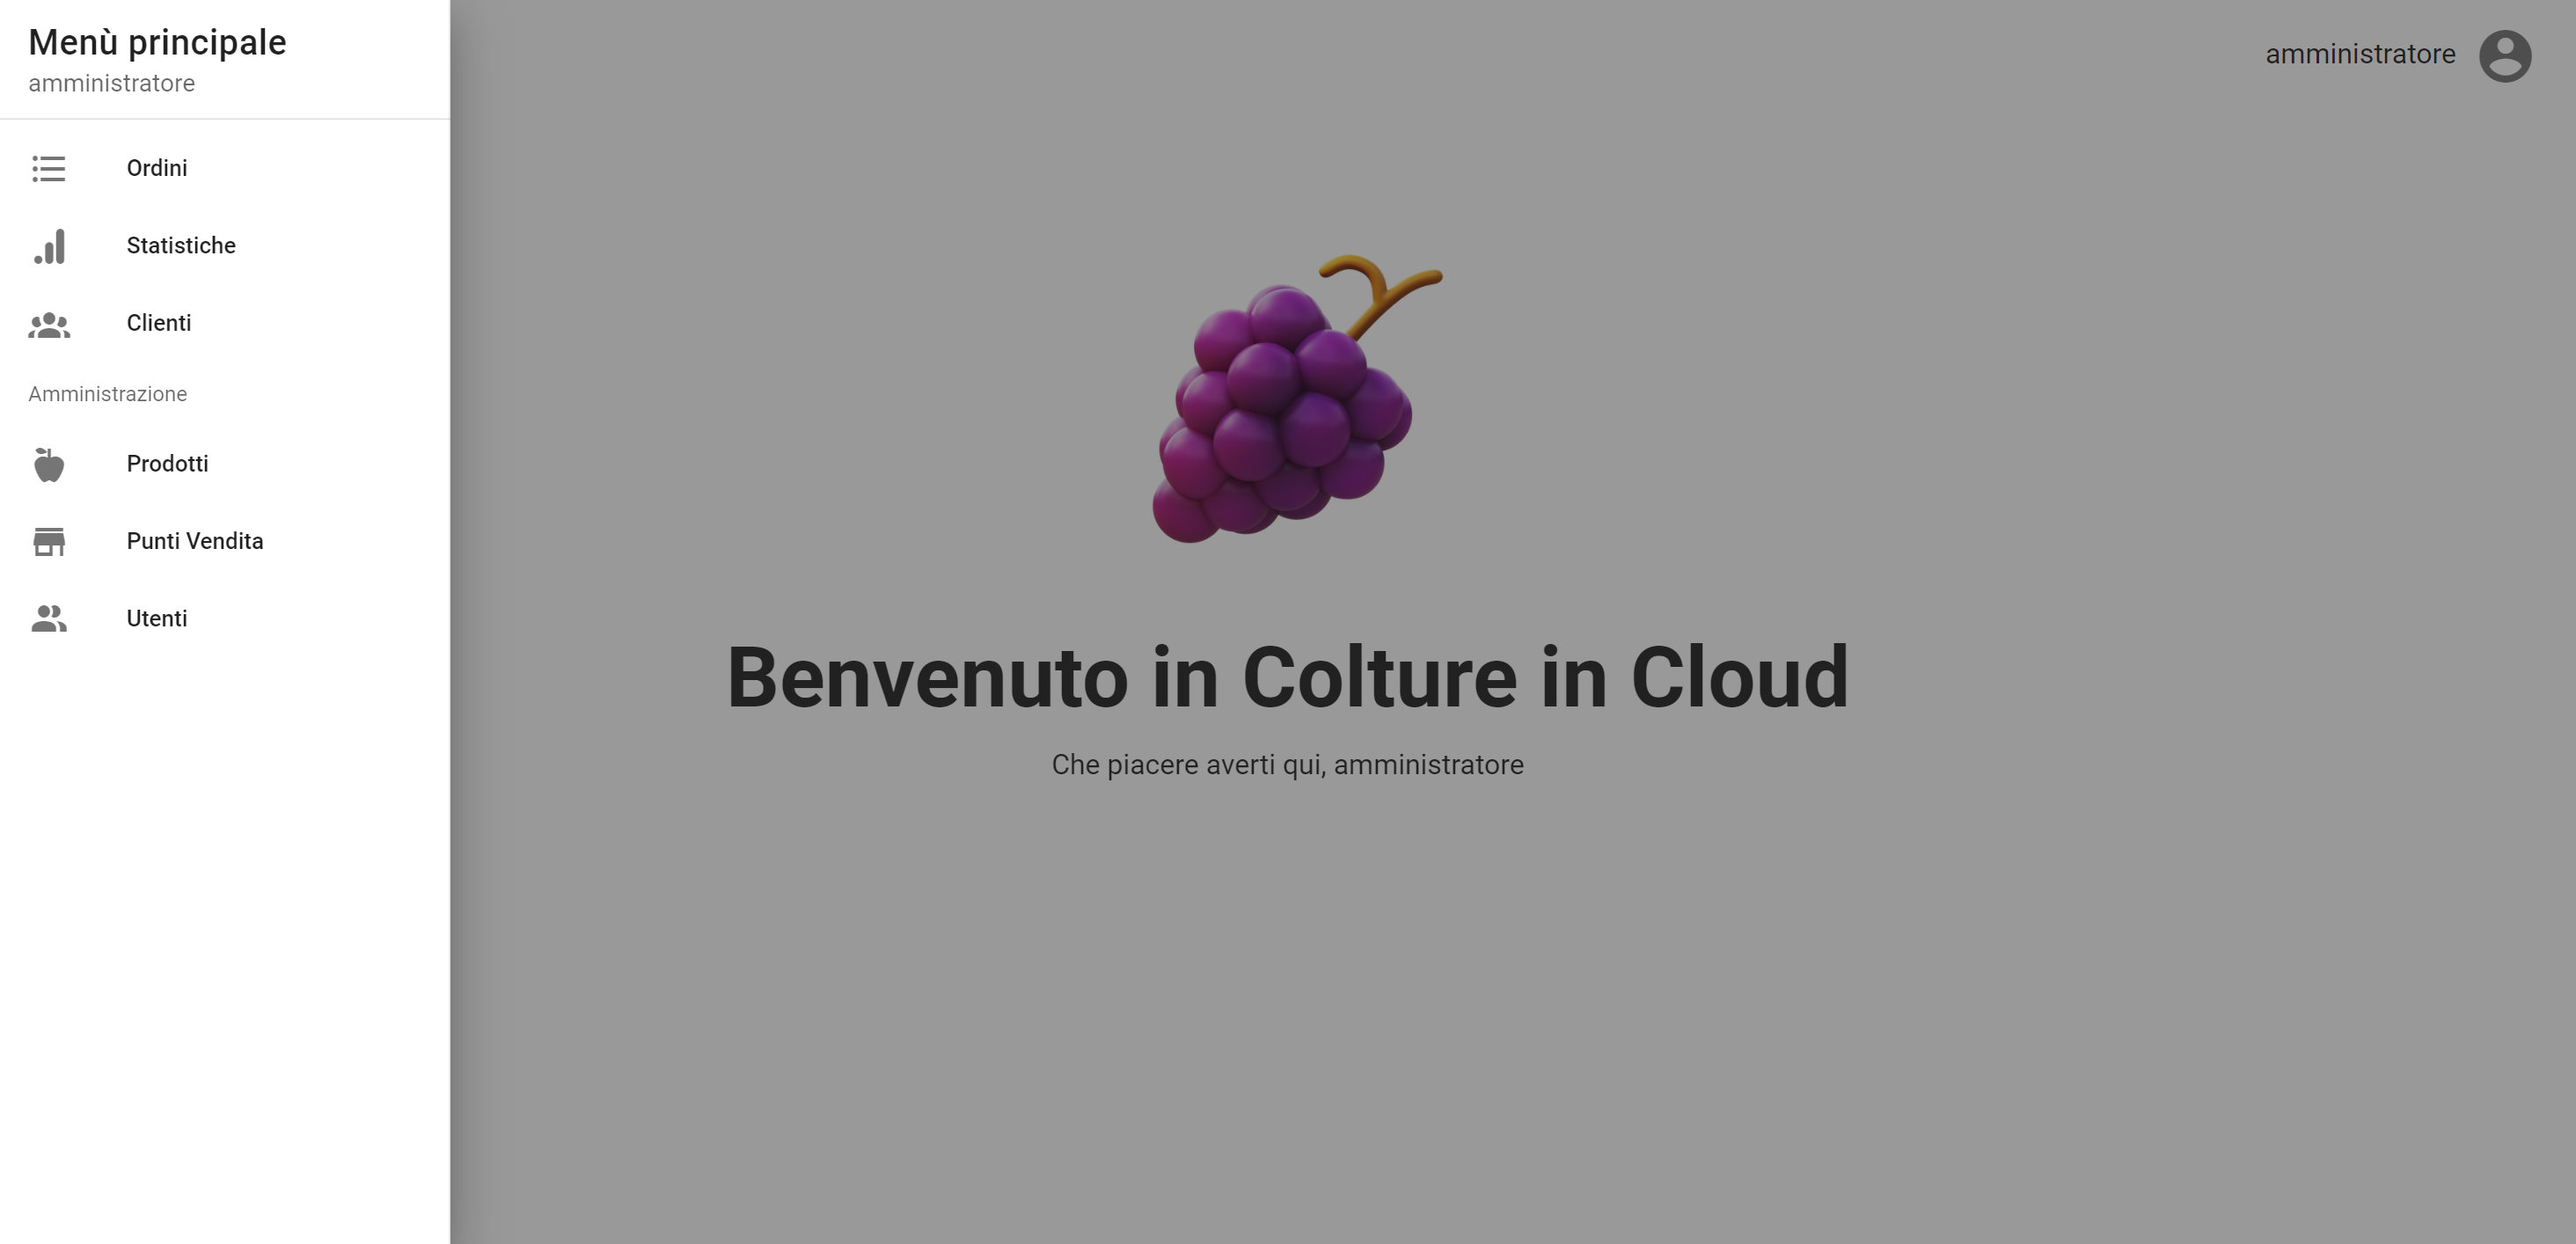
\includegraphics[width=\textwidth]{assets/final_menu.png}
    \caption{Menù principale visibile da un utente con privilegi di amministratore}
    \label{fig:menu}
\end{figure}
\newpage
Nella pagina ordini è possibile visualizzare la lista degli ordini a cui un utente ha accesso con la possibilità di filtrare per punto vendita e periodo di tempo; per ogni ordine è possibile visualizzare il dettaglio, modificarlo e cancellarlo.
\begin{figure}[htp]
    \centering
    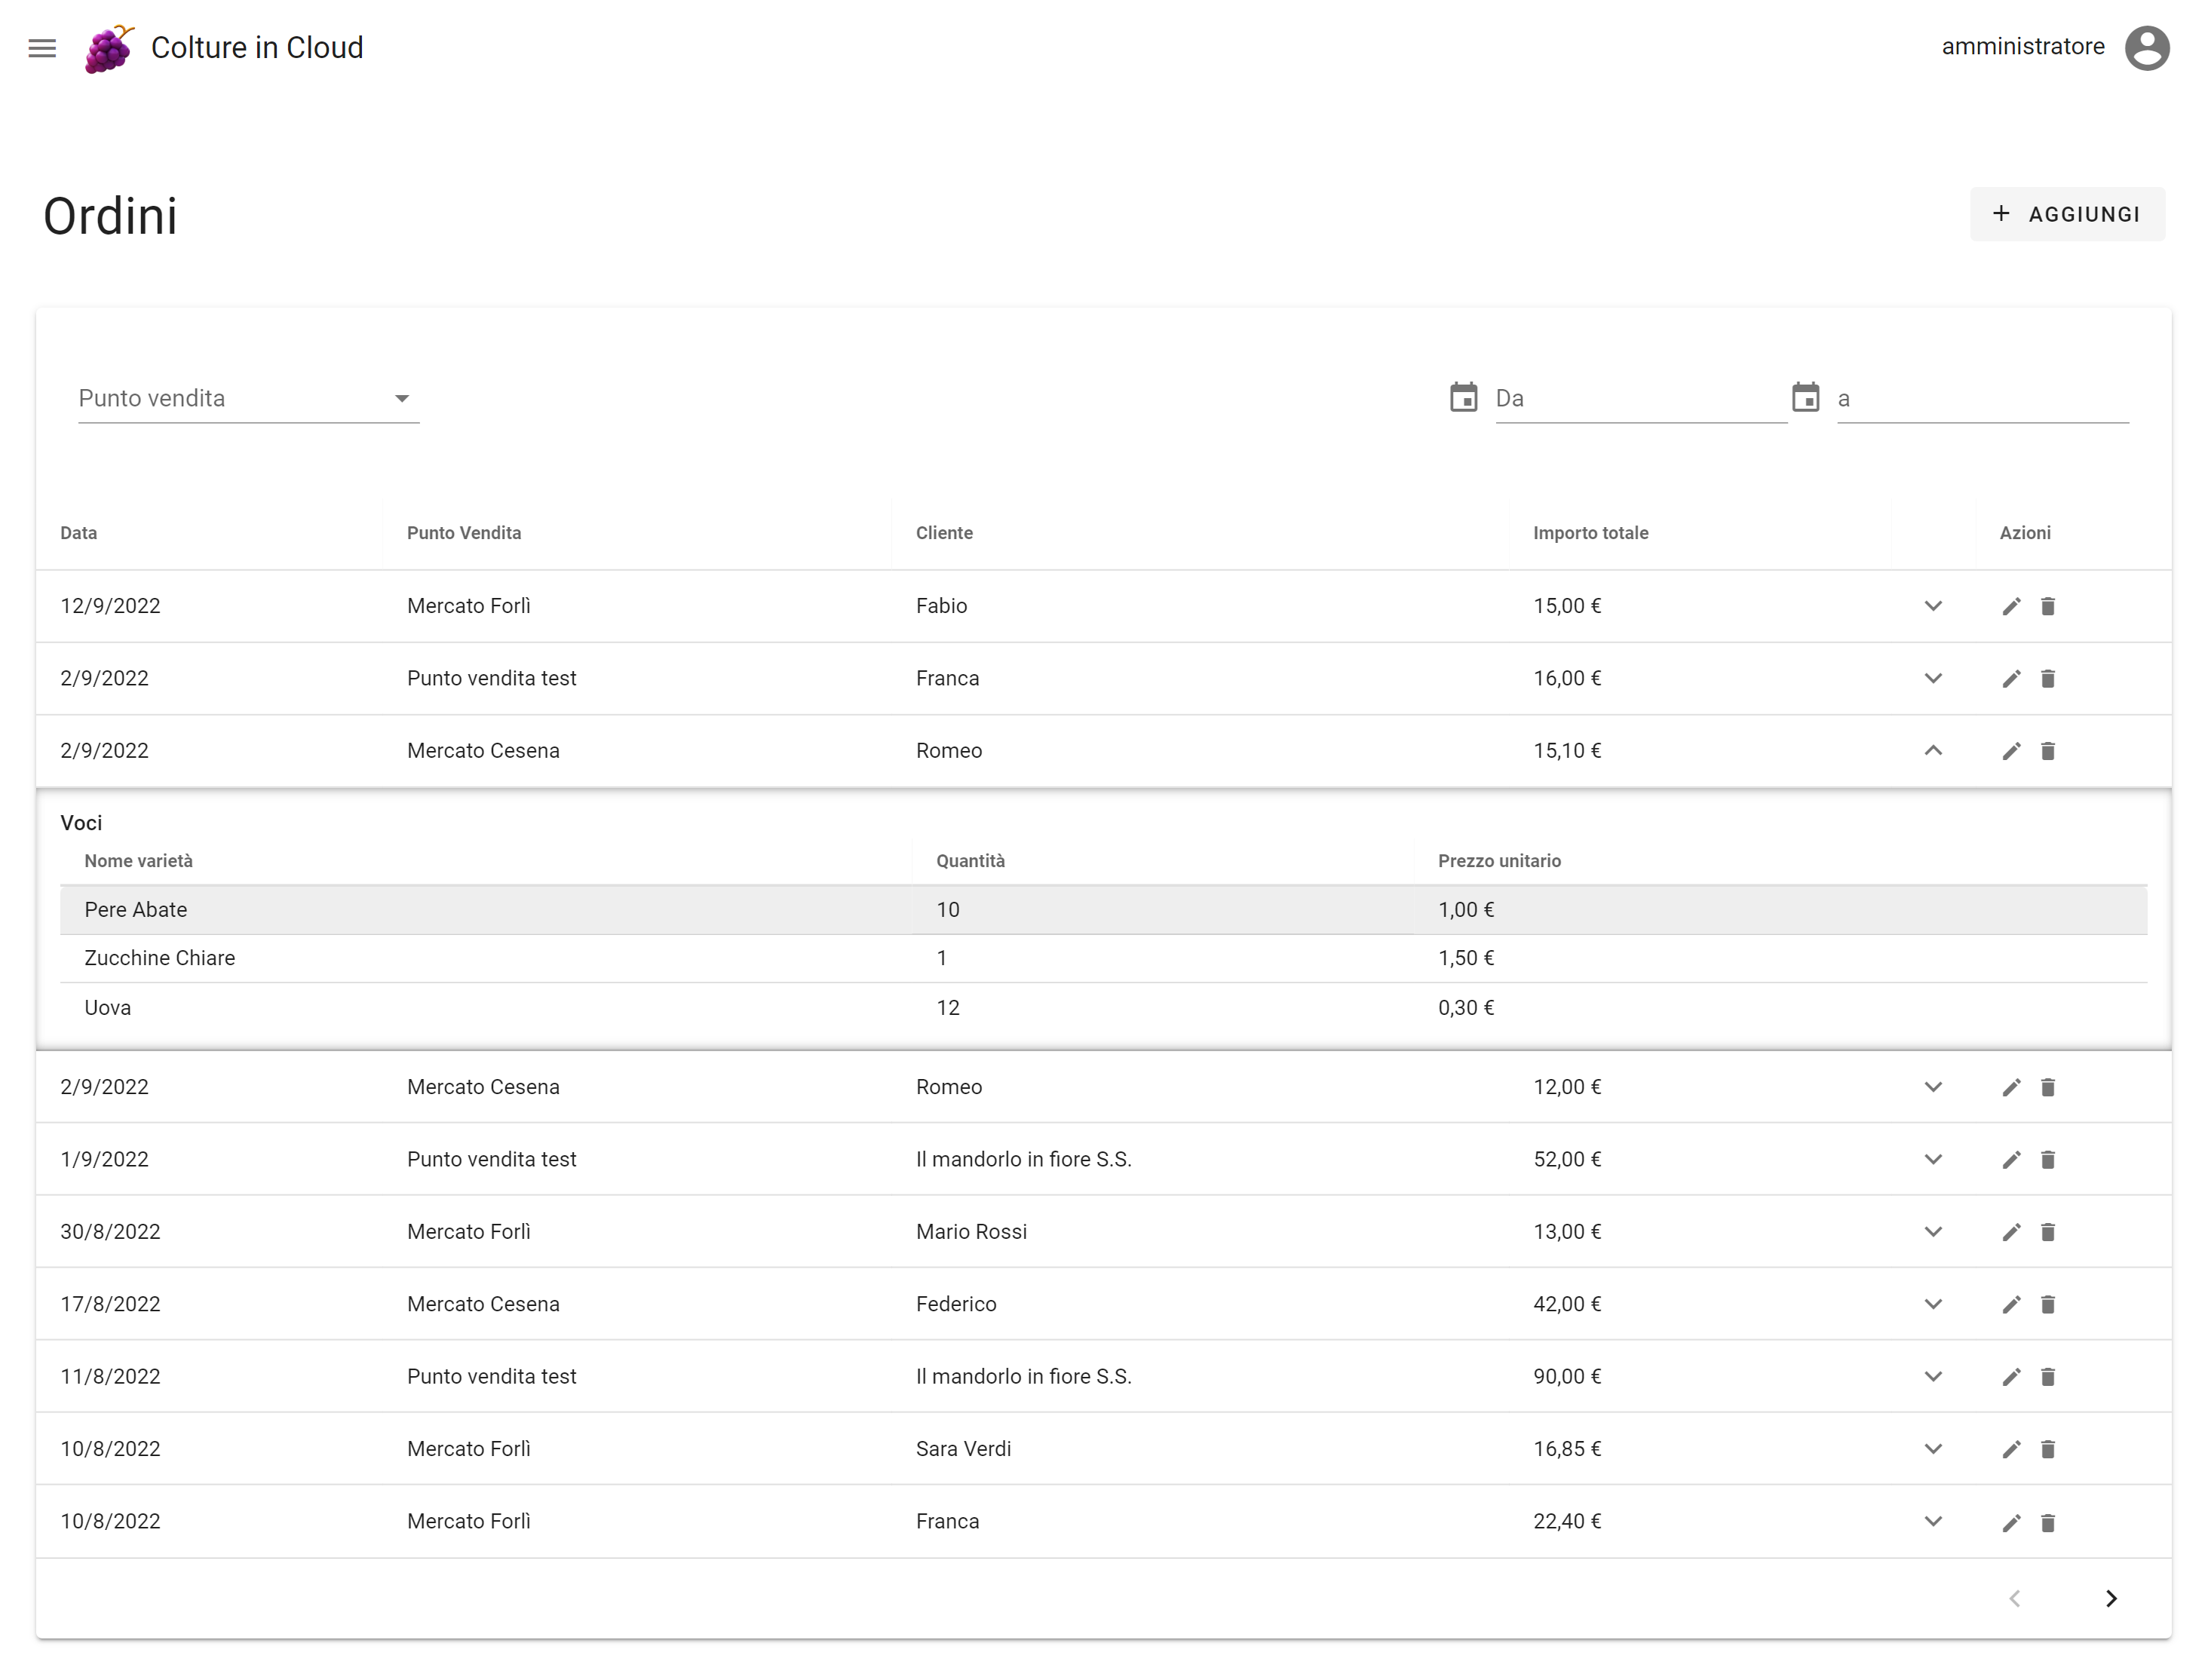
\includegraphics[width=\textwidth]{assets/final_orders.png}
    \caption{Visualizzazione pagina ordini}
    \label{fig:order_page}
\end{figure}
\newpage
Il pulsante \textit{aggiungi} apre un form in cui inserire i dati del nuovo ordine.
\begin{figure}[htp]
    \centering
    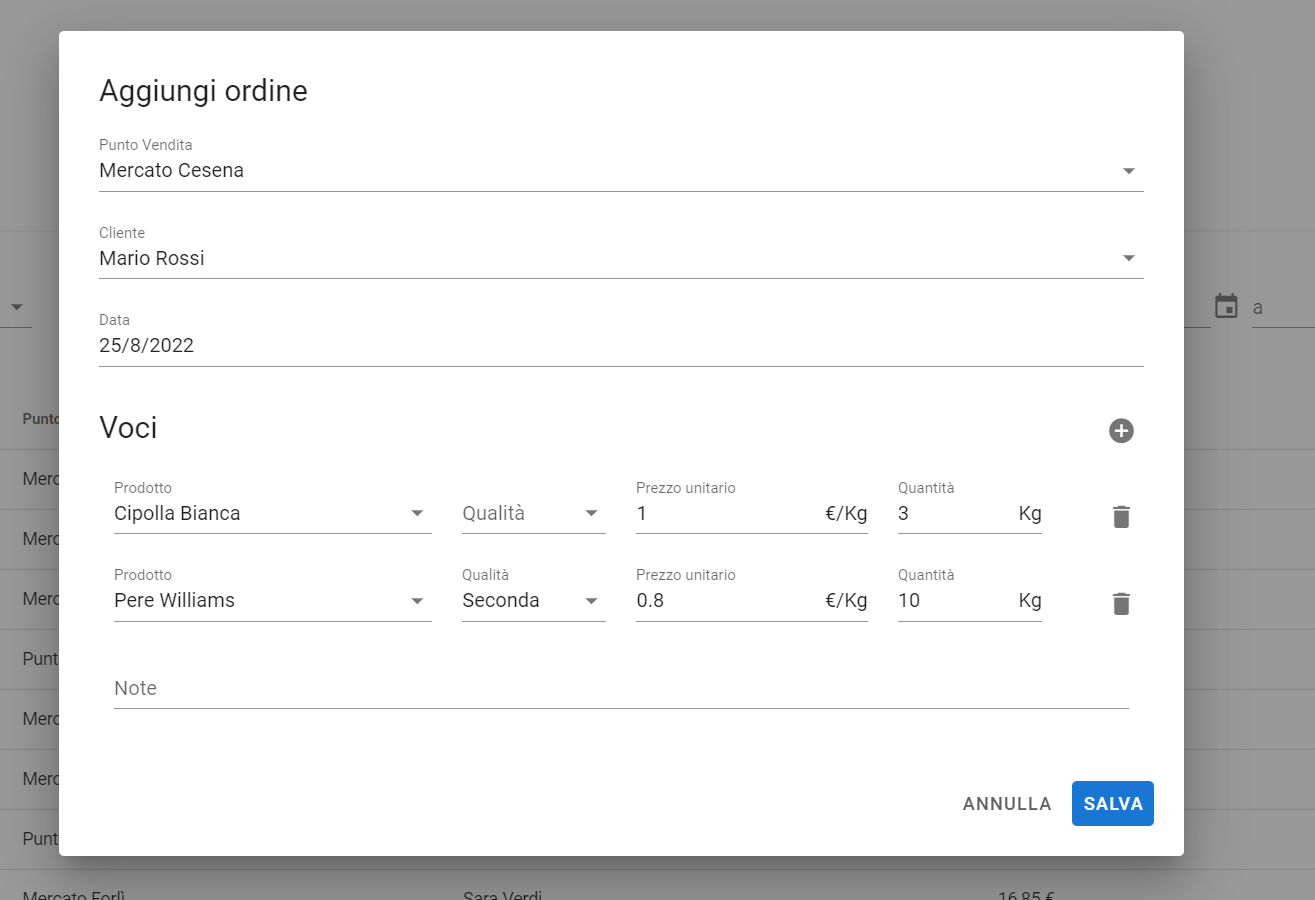
\includegraphics[width=\textwidth]{assets/final_add_order.png}
    \caption{Visualizzazione funzione aggiungi ordine}
    \label{fig:addOrderForm}
\end{figure}

Nella pagina statistiche si possono vedere i grafici relativi alle vendite con la possibilità di filtrare in base ai dati di interesse.
\begin{figure}[htp]
    \centering
    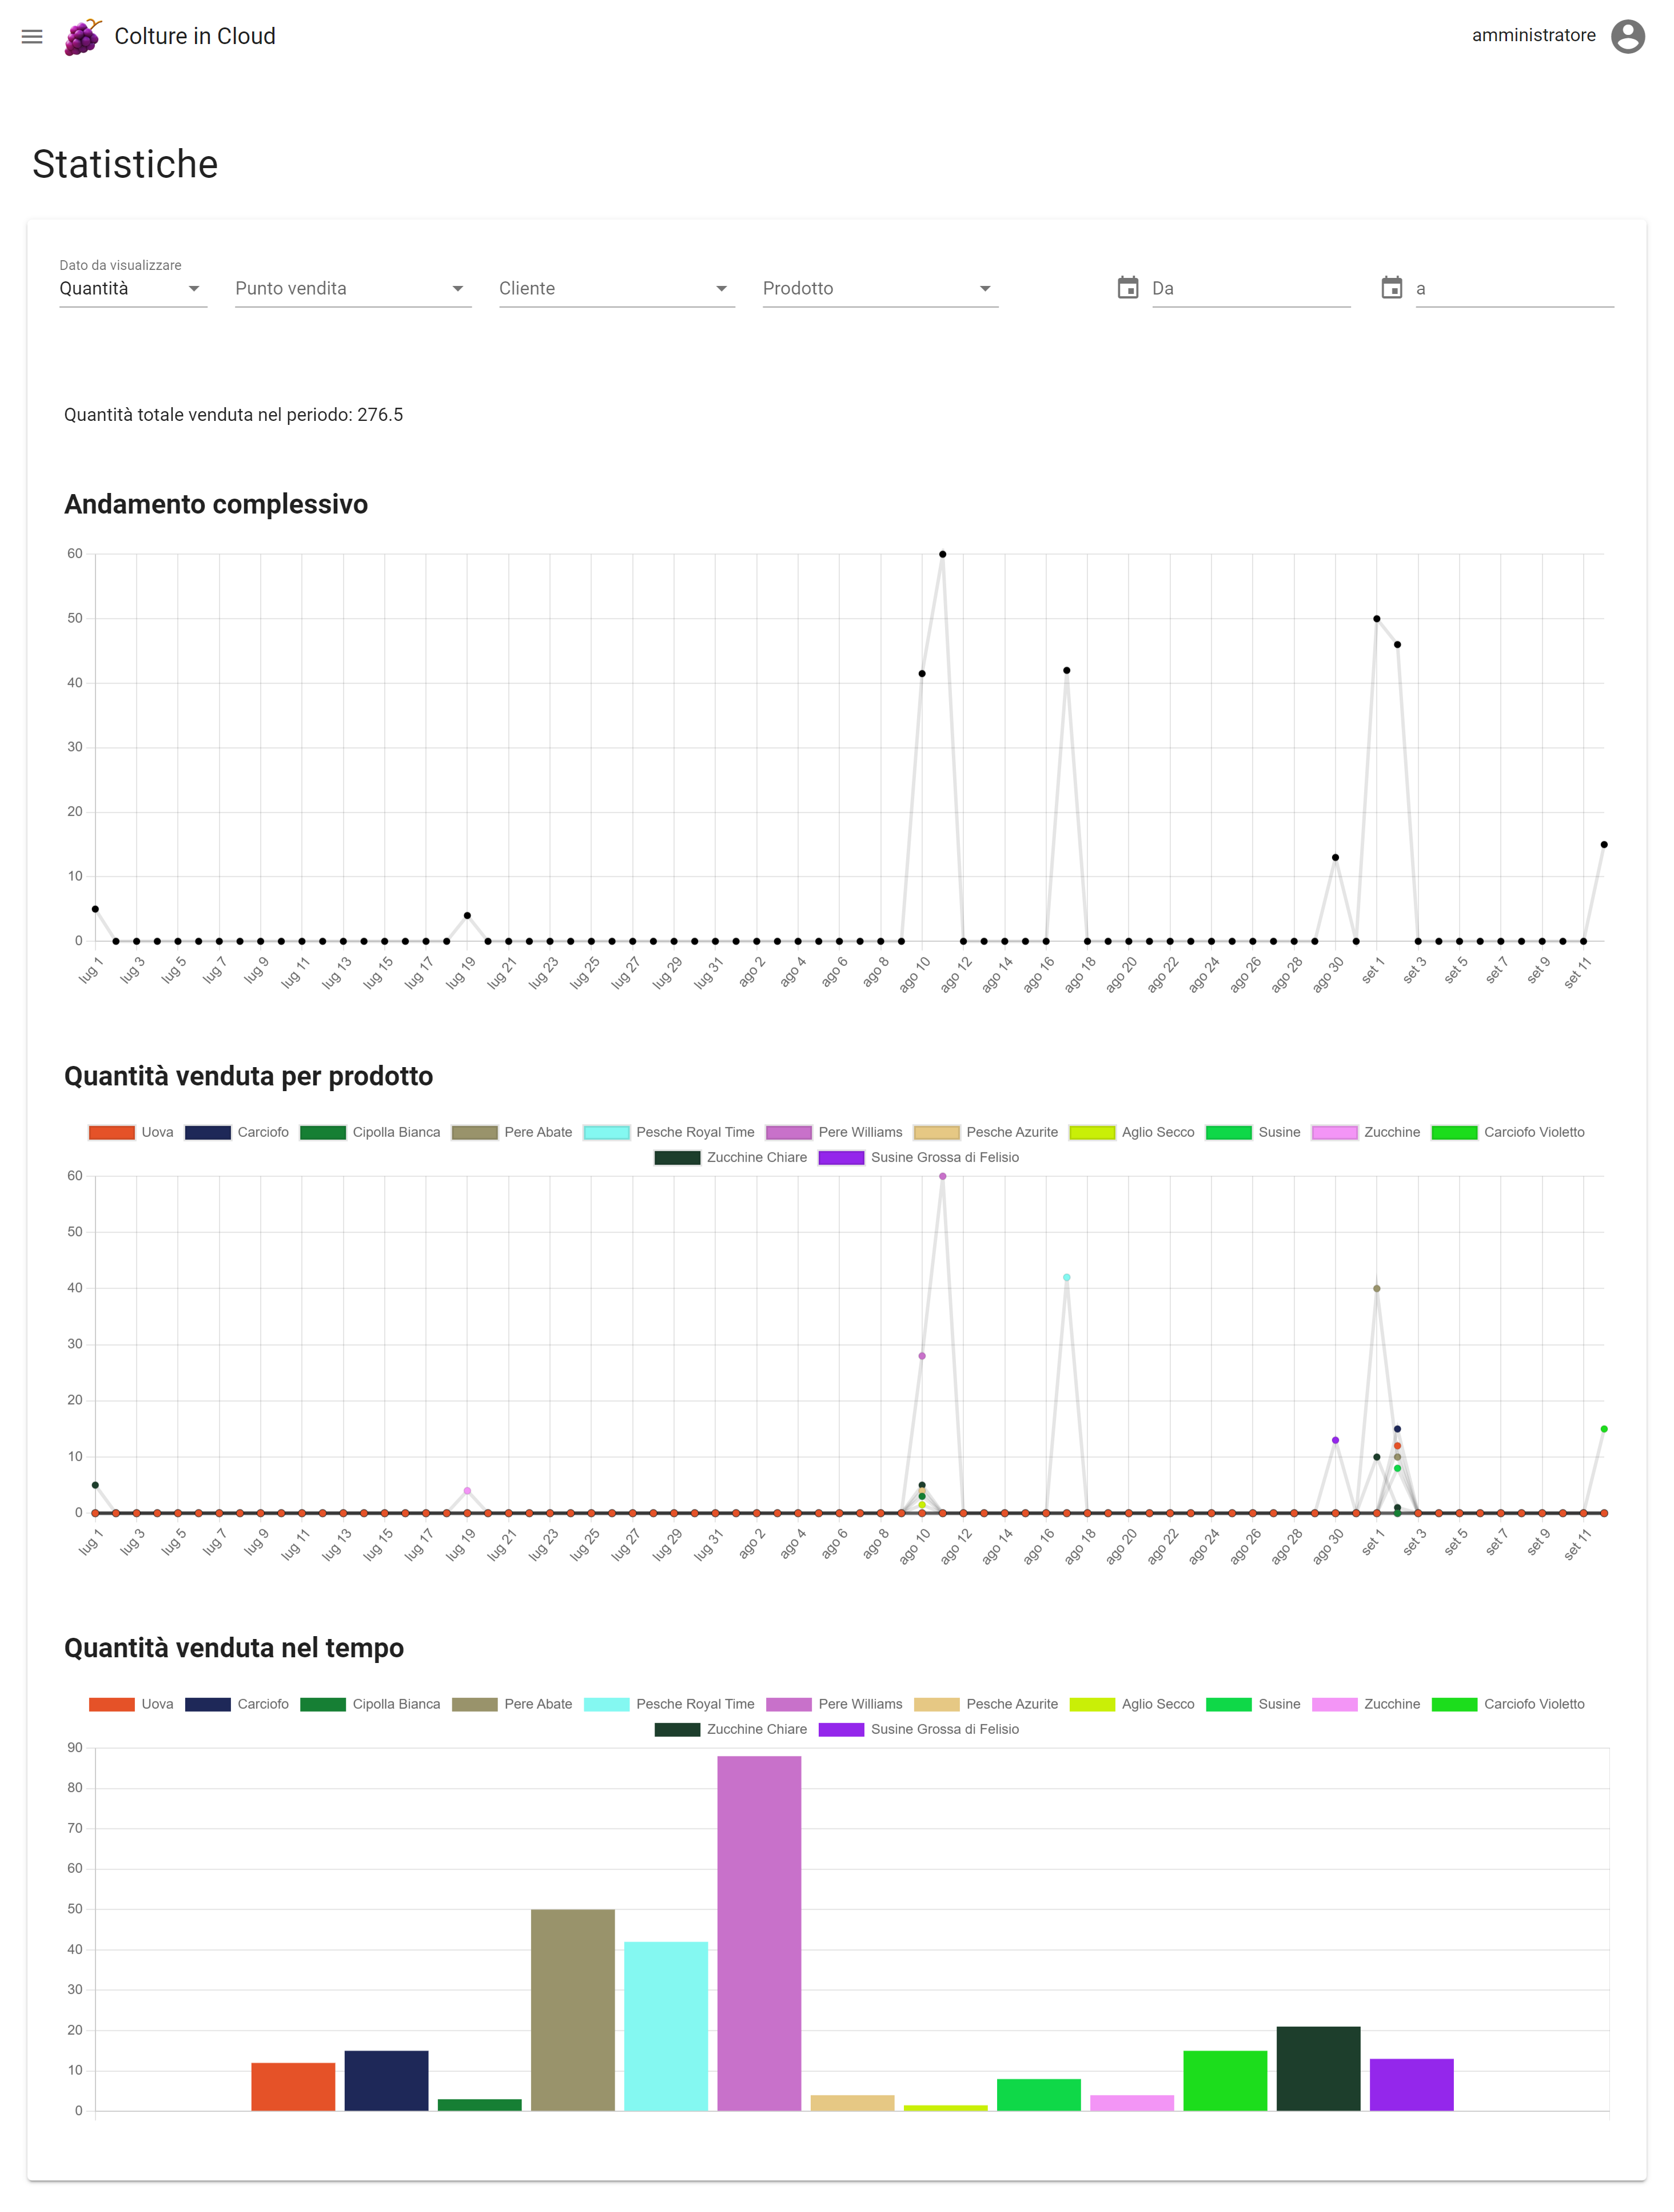
\includegraphics[width=\textwidth]{assets/final_stats.png}
    \caption{Visualizzazione statistiche}
    \label{fig:stats}
\end{figure}
\newpage
Le altre pagine relative a clienti, prodotti, punti vendita e utenti, presentano tutte la stessa struttura con l'elenco degli elementi e la possibilità di aggiungerne di nuovi, modificare o cancellare quelli presenti.
\begin{figure}[htp]
    \centering
    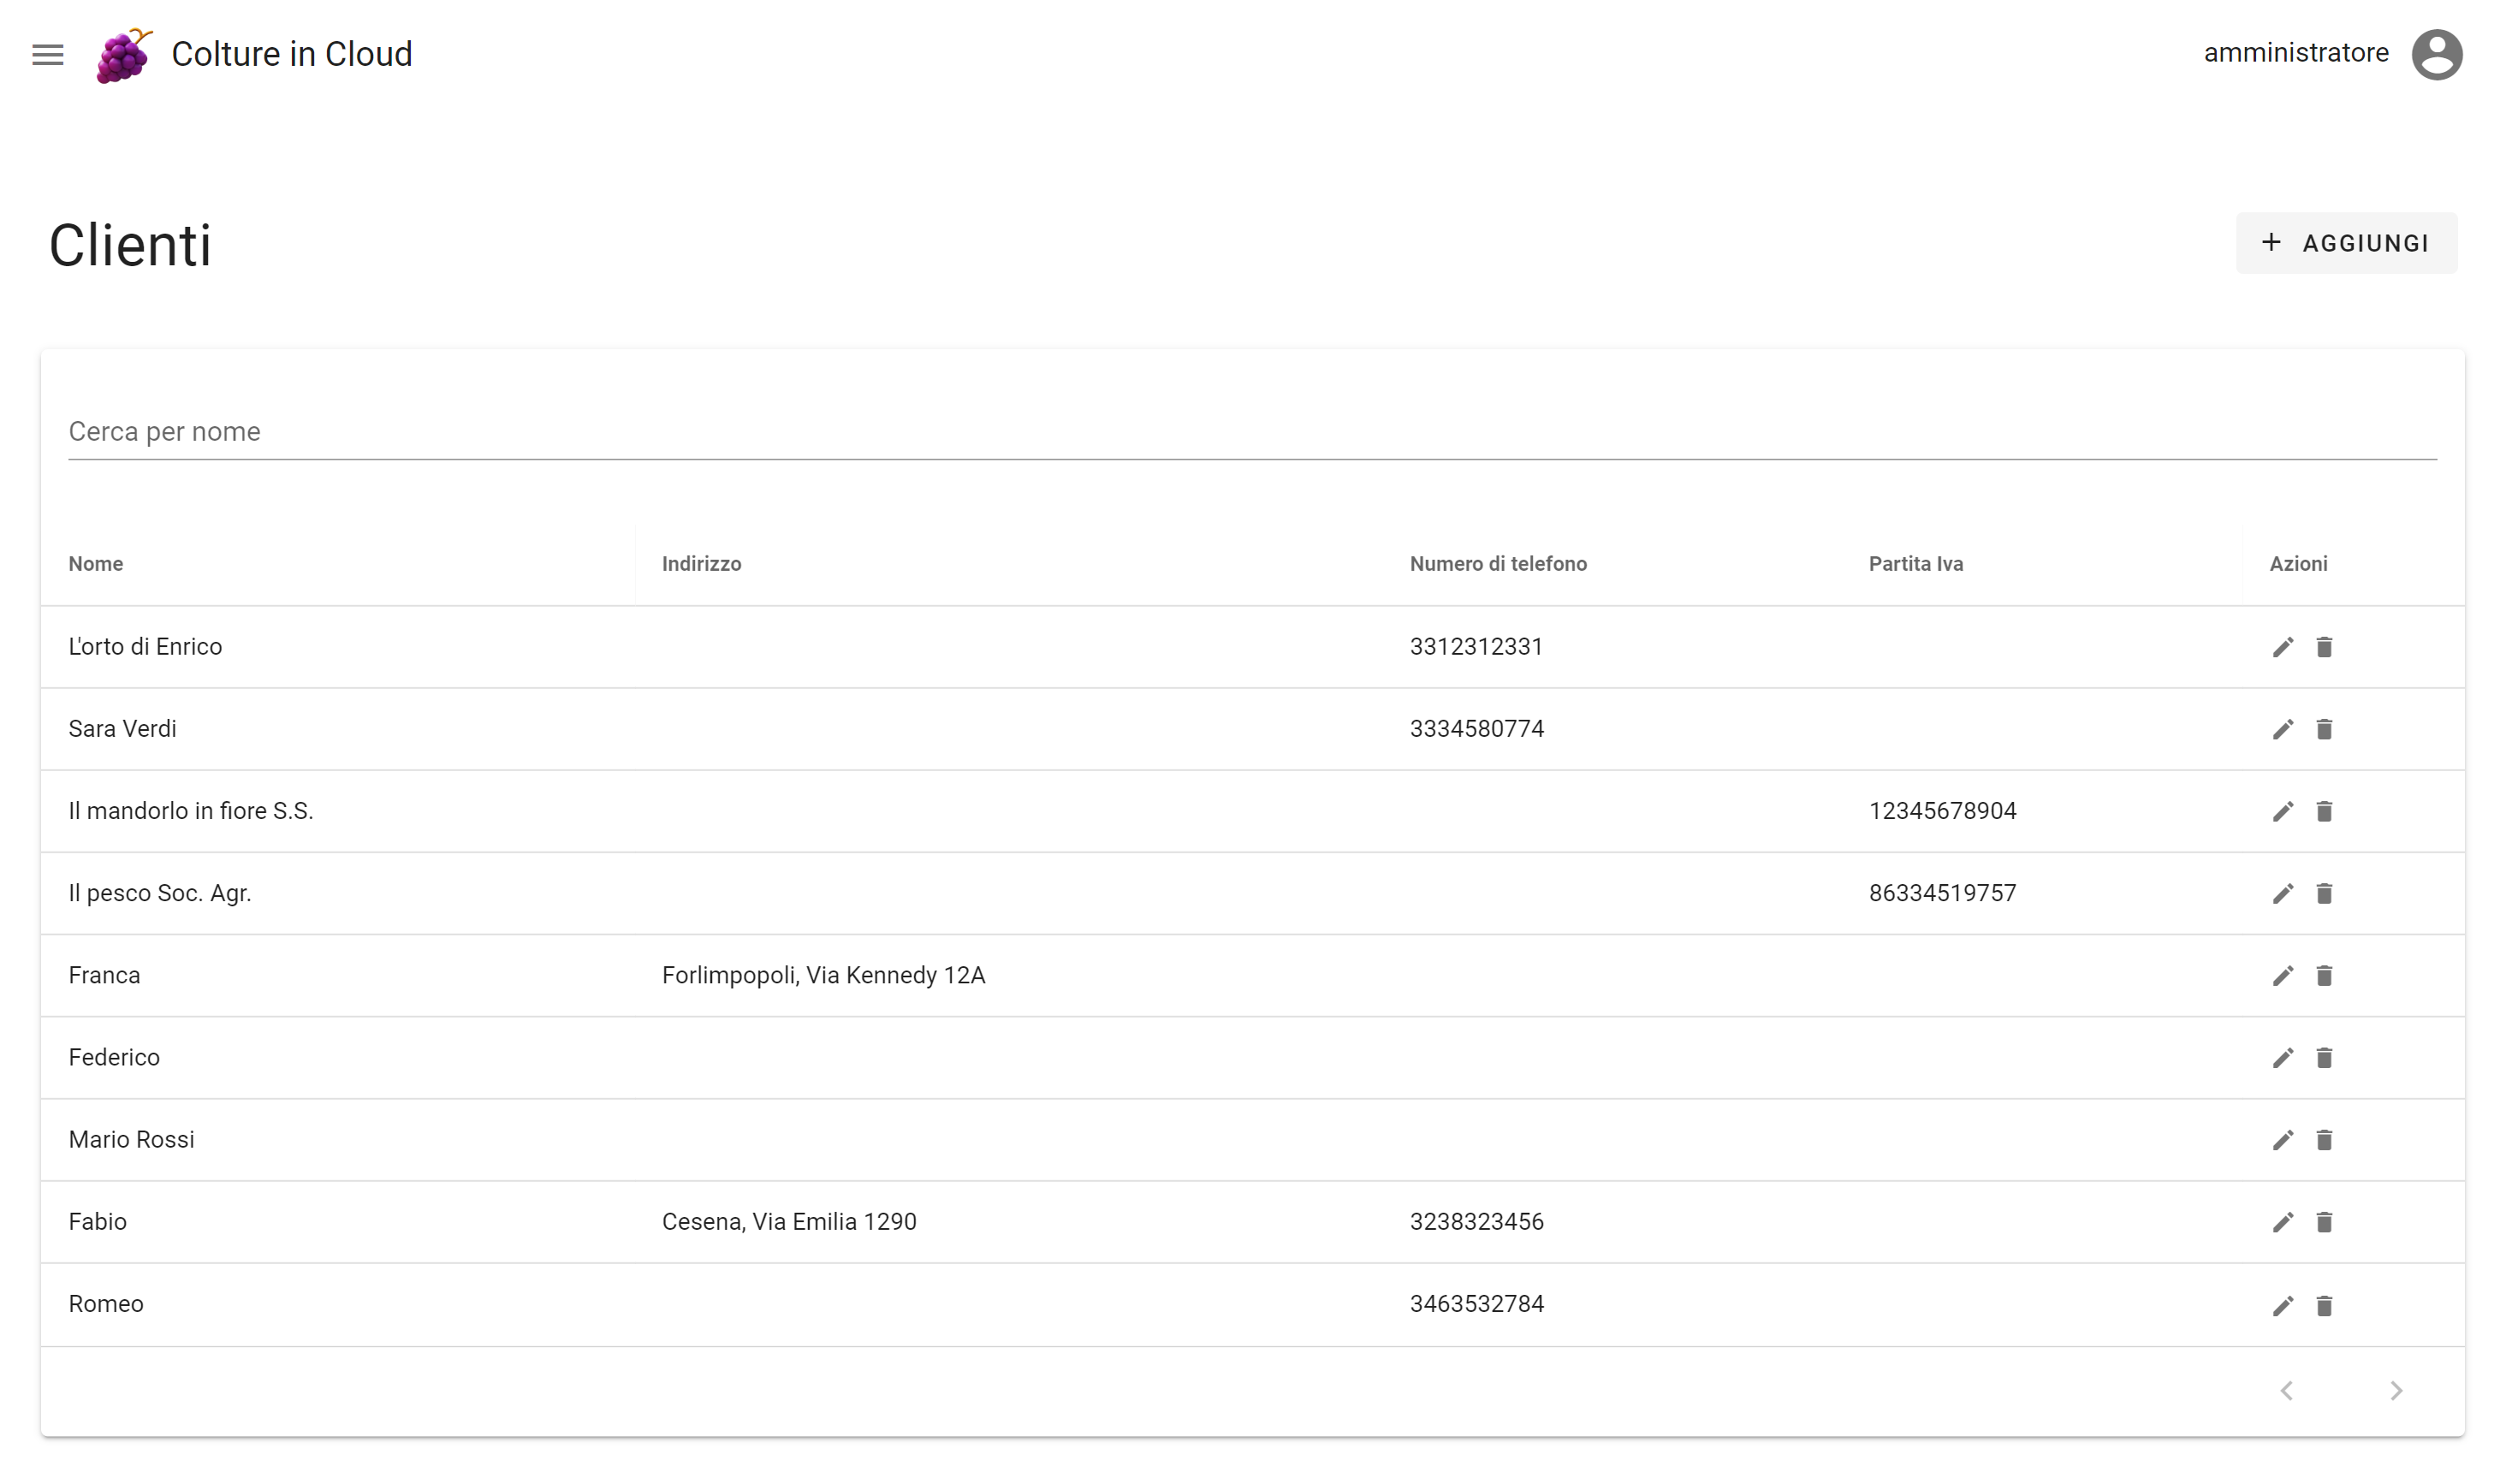
\includegraphics[width=\textwidth]{assets/final_customers.png}
    \caption{Visualizzazione pagina clienti}
    \label{fig:client_page}
\end{figure}
\begin{figure}[htp]
    \centering
    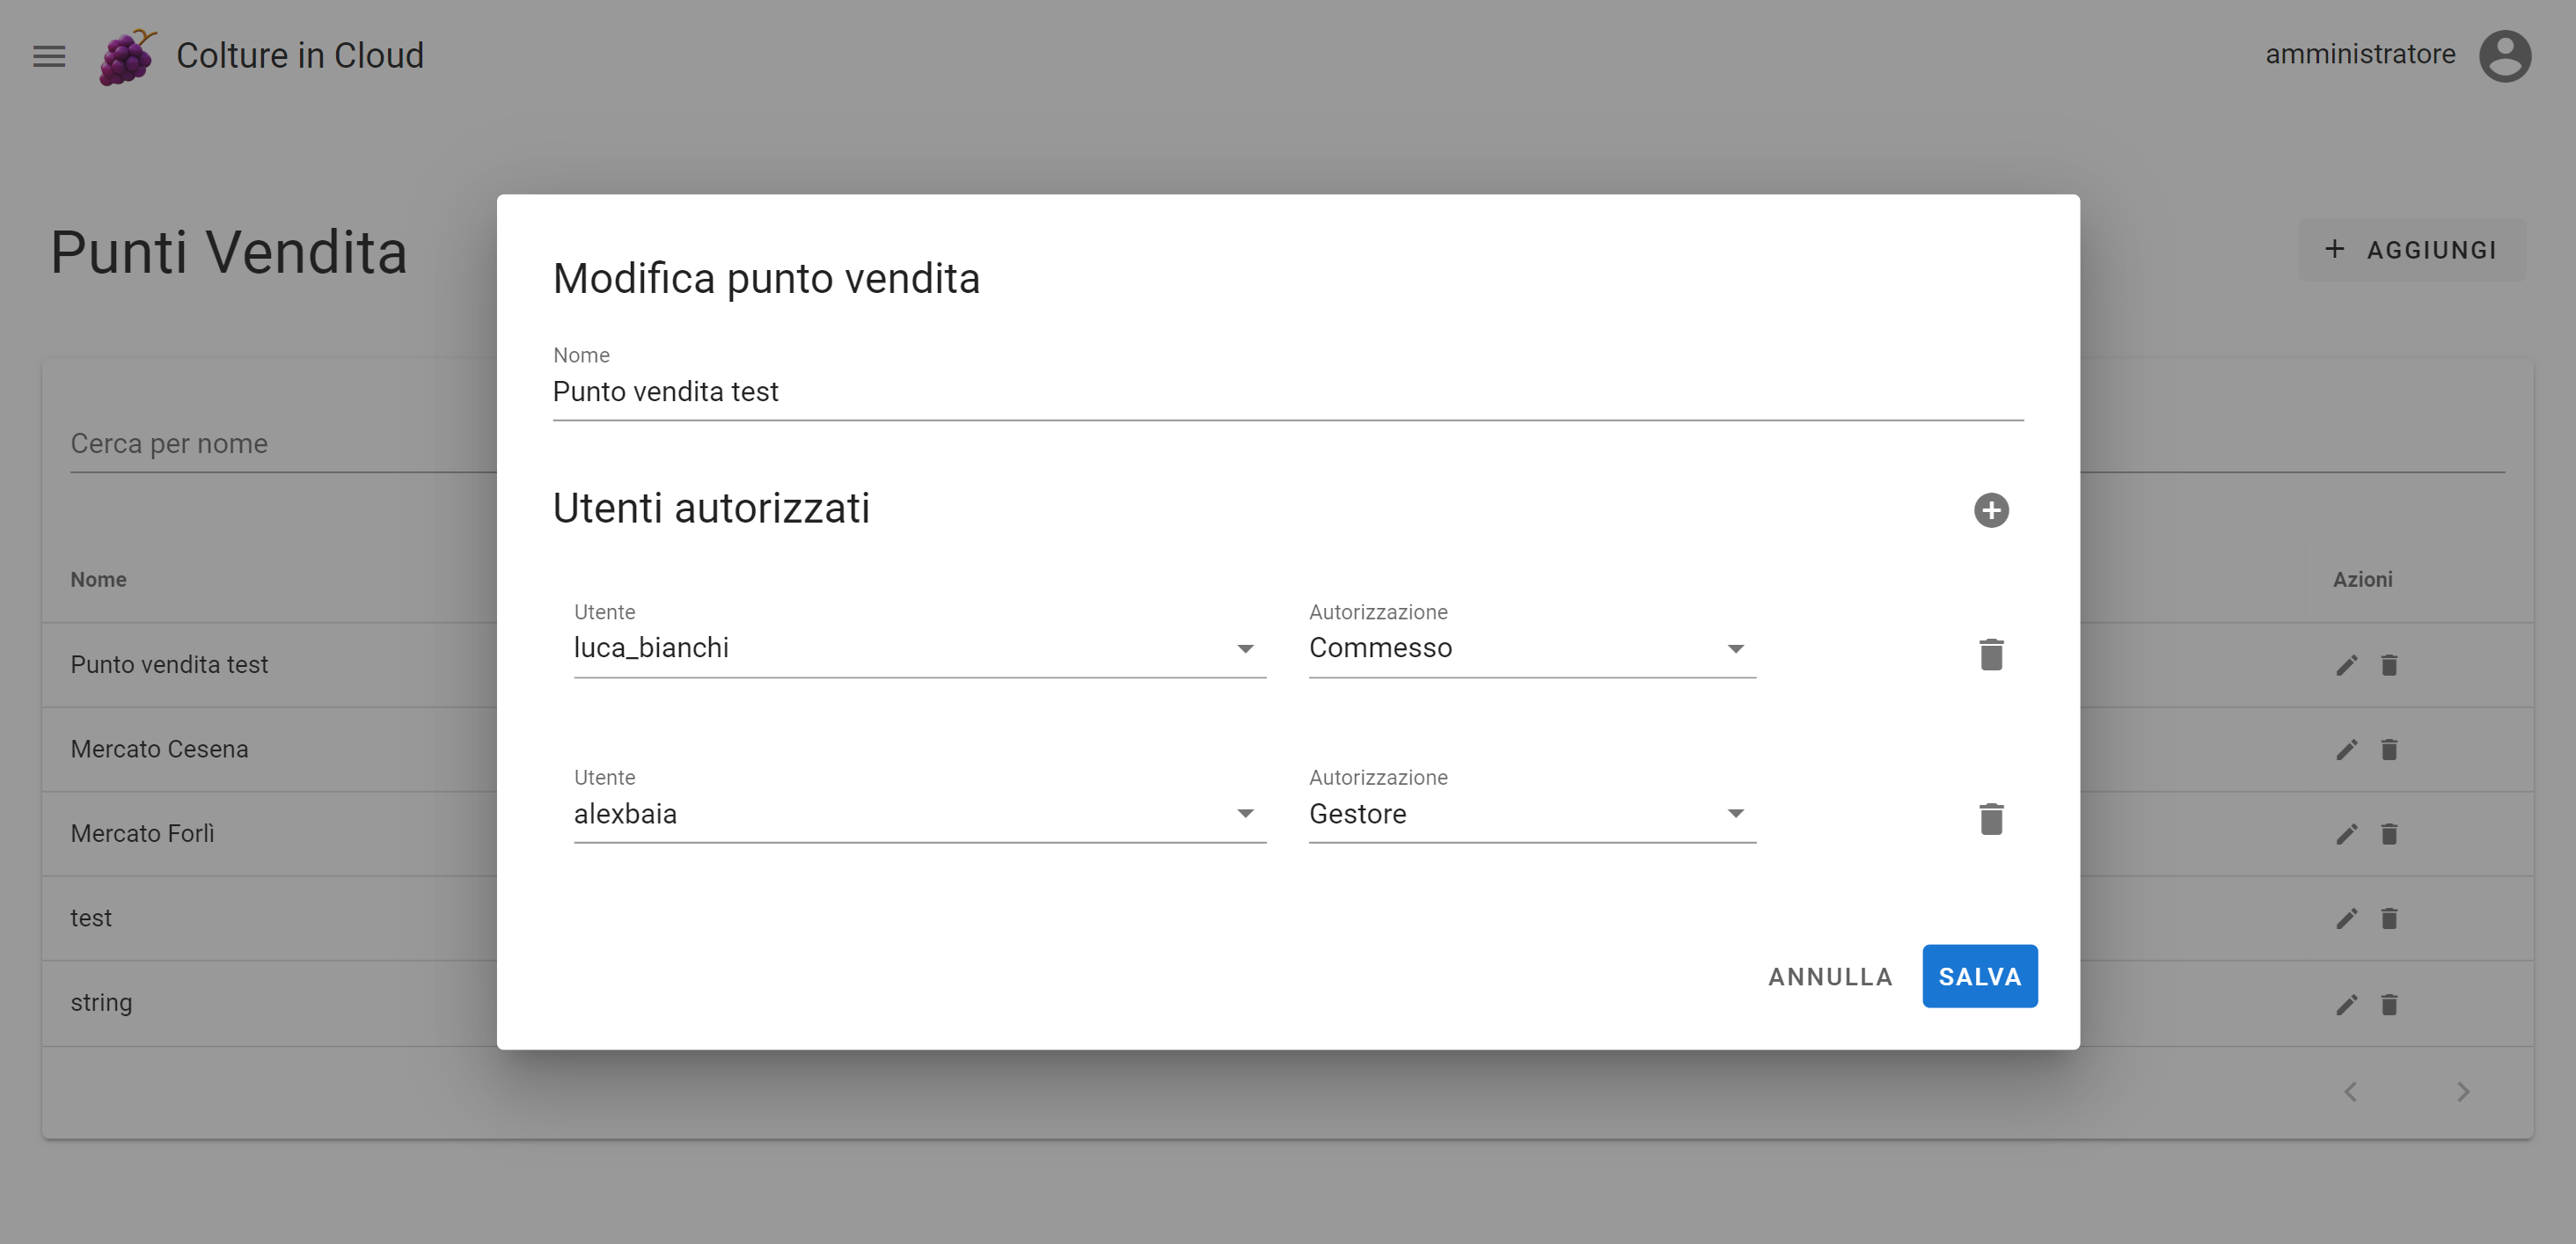
\includegraphics[width=\textwidth]{assets/final_edit_store.png}
    \caption{Visualizzazione modifica di un punto vendita}
    \label{fig:stores}
\end{figure}
\begin{figure}[htp]
    \centering
    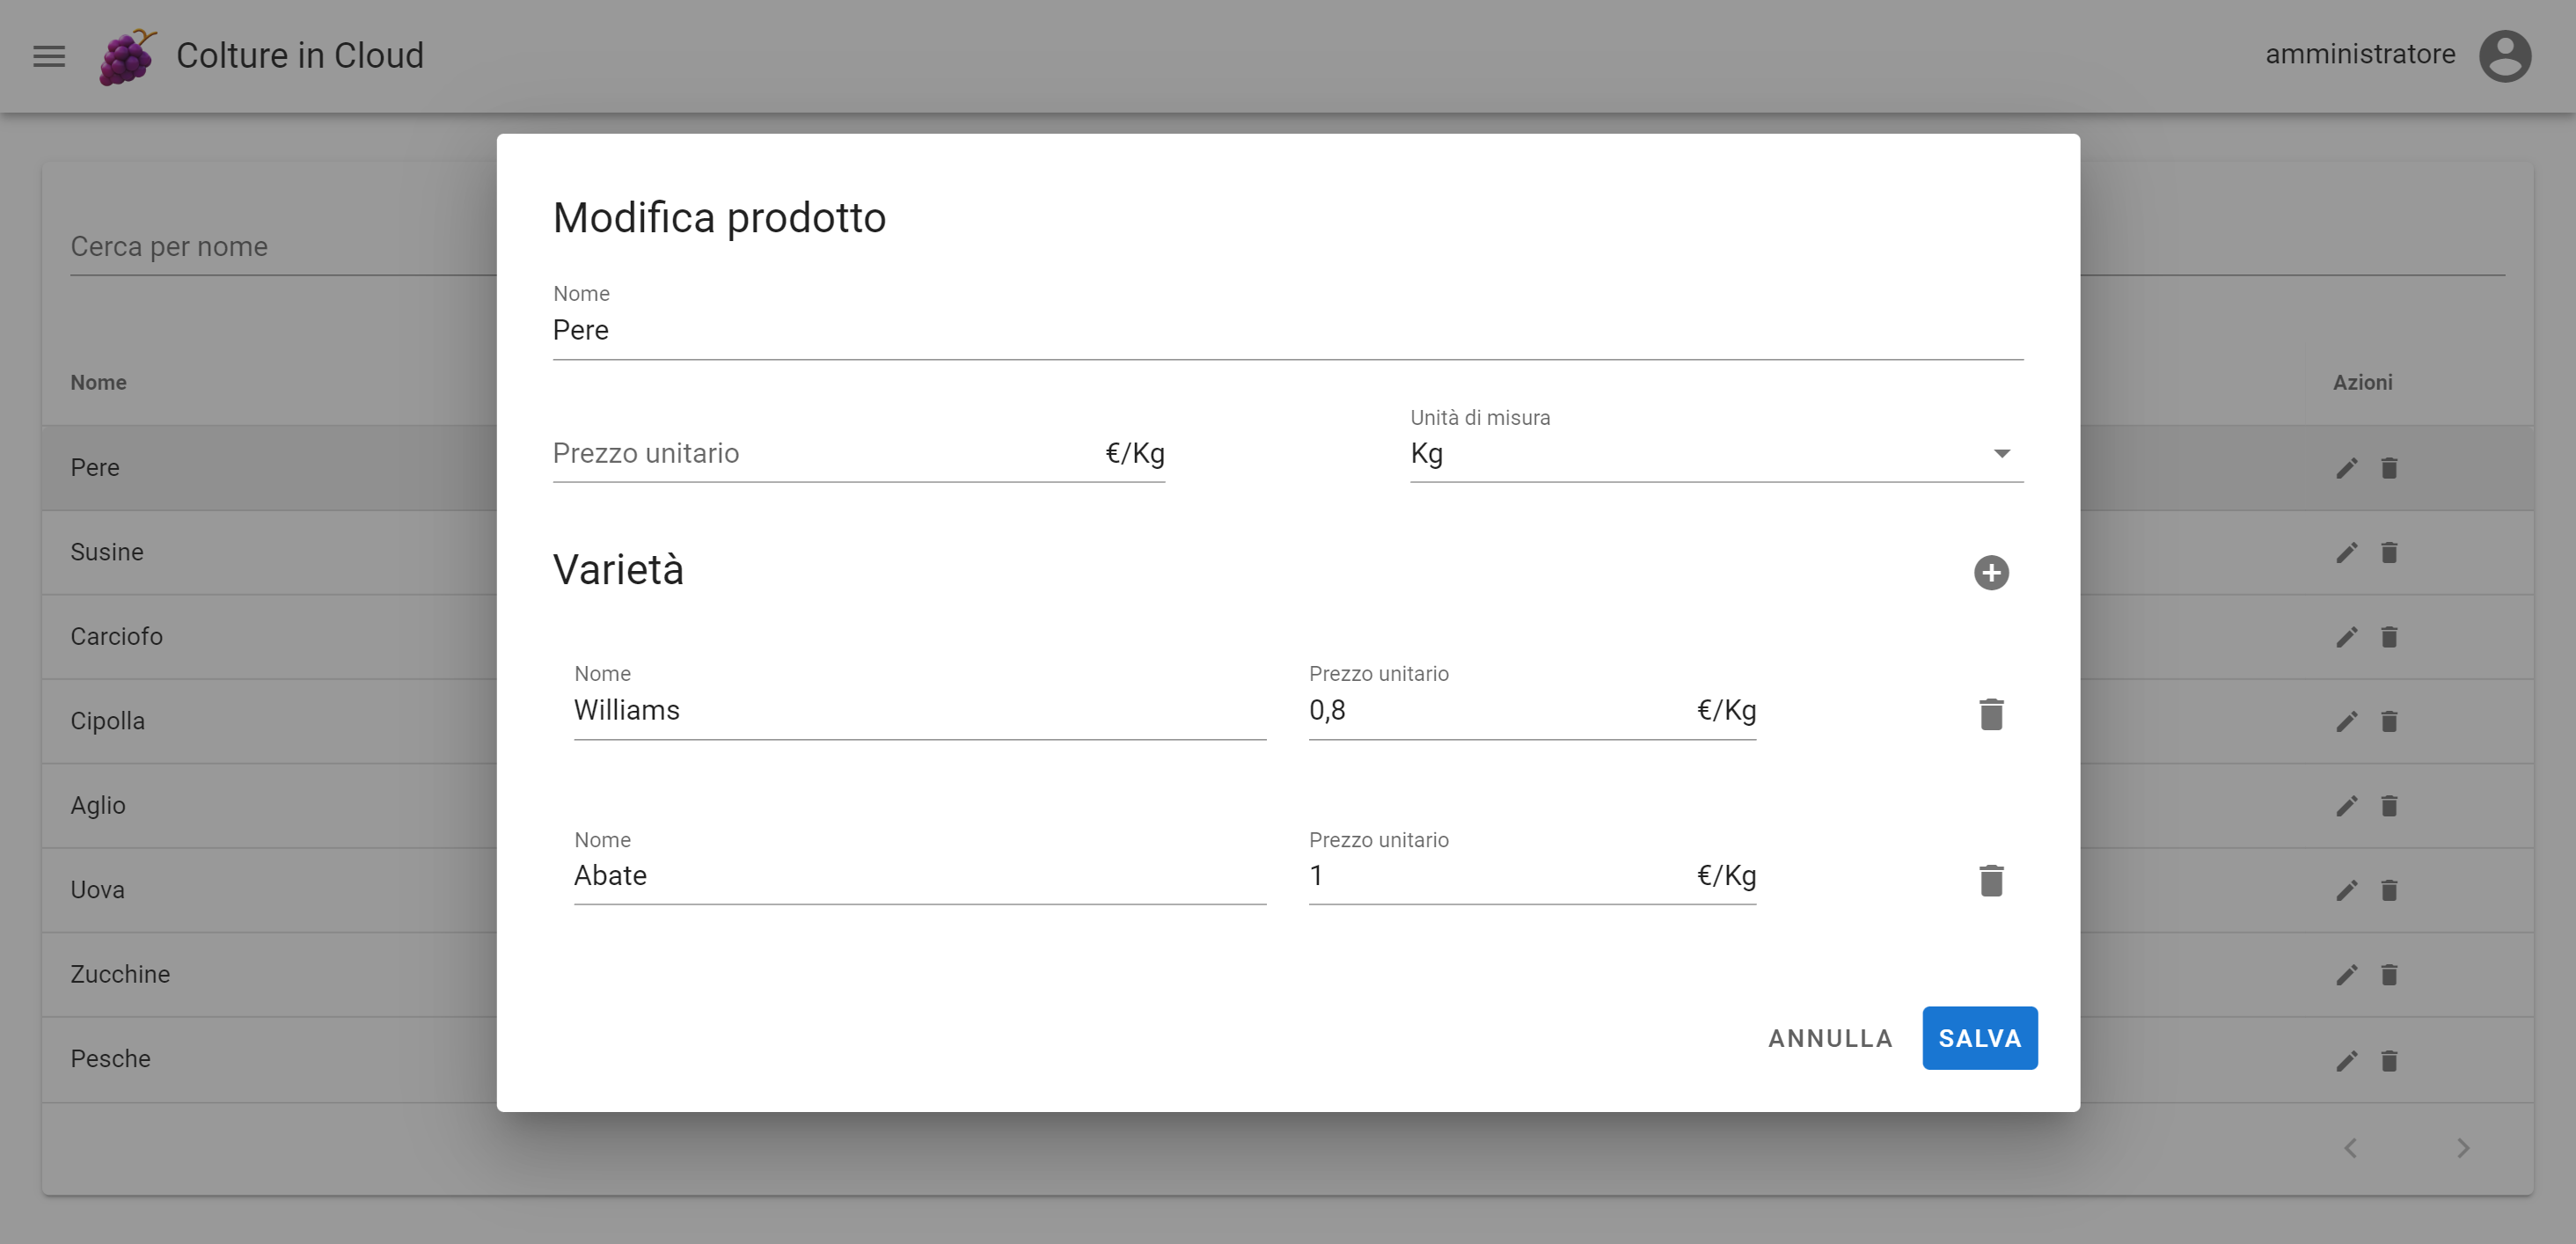
\includegraphics[width=\textwidth]{assets/final_edit_product.png}
    \caption{Visualizzazione modifica di un prodotto}
    \label{fig:updateProduct}
\end{figure}

\chapter{Conclusioni}
La soluzione proposta soddisfa tutti i requisiti che erano stati prefissati e ciò rappresenta una bella soddisfazione per il team.
L'applicazione realizzata ha ancora margini per essere perfezionata attraverso estensioni che potranno essere aggiunte in futuro, le quali emergeranno anche dalle opinioni degli utenti che utilizzeranno quotidianamente l'applicazione. In particolare si può già pensare di migliorare la sezione statistiche per una analisi sempre più approfondita e dettagliata dei dati. Inoltre, sarà interessante procedere alla messa in uso del sistema integrando i dati attualmente posseduti dall'azienda, attraverso apposita migrazione.
\section{Commenti finali}
Il team ritiene che la progettazione e lo sviluppo di questo progetto sia stata molto interessante e stimolante, in quanto rappresenta uno scenario d'uso reale in cui mettere in pratica ciò che è stato affrontato a lezione e toccare con mano le criticità e i problemi che si devono affrontare. Inoltre, è stato possibile vedere come nonostante l'idea iniziale del progetto sembrasse semplice da realizzare, ci si è presto resi conto che gli elementi da tenere in considerazione e da sviluppare non fossero poi così pochi e portarli tutti a termine necessita di tempo e lavoro. 

\end{document}
